\chapter{Theoretical background}\label{cap.theoretic}

In this chapter we explain the theoretical concepts of our work, this includes the theory of tracking and person re-identification.

\section{Tracking}


As we explained in previous chapters, there are a traditional family of methods to solve the tracking problem. But with the incursion of deep learning techniques, they have been adapted to it and create new paradigms. The main ways to apply deep learning techniques to tracking are the following \cite{thrun}:


\begin{itemize}


\item \textbf{Tracking-by-detection}. These methods use a specific class classifier and there is not need to train it online. So, these methods use a neural network to extract instances of the frames and then linked with temporal restrictions. 

\item \textbf{Tracking learning and detection}. Starting from the first frame of a video, a tracker will sample patches near the target object, and they are used to train a foreground-background  classifier, and this classifier is used to score patches from the next frame to estimate the new location of the target object. These methods showed a state-of-the-art performance results. Unfortunately, neural networks are slow to train, therefore the speed of the method is reduced \cite{deep1} \cite{deep2}.


\item \textbf{Siamese based tracking}. In this approach, many candidate patches are passed through the network, and the patch with the highest matching score is selected as the tracking output \cite{trackingSiamese}.


\item \textbf{Tracking as regression}, these methods are an extension of object localization using neural networks, these methods given an image containing an object predict the bounding box which contain the object in every frame \cite{thrun}. They are restricted to one object.


\item \textbf{Tracking with RNN}. From the output of an object detector, these tracking algorithms model the sequence of movement of objects using an recurrent neural network \cite{savaresee}. These methods represent the current state of art in tracking.


\end{itemize}



\subsection{Tracking-by-detection}

For this thesis we chose the tracking-by-detection paradigm. We get the detections with a object detector based on deep learning networks, and we link those detections with a tracking by matching, particularly, tracking by feature.

\subsubsection{Detection in tracking}\label{trackingBounding}


In object detection too, the emergence of the neural networks has supposed a turning point. As we can observe in \ref{deepObjet}, the mean average precision, has almost doubled since the appearance of deep neural networks.


\begin{figure}[H]
\centering         
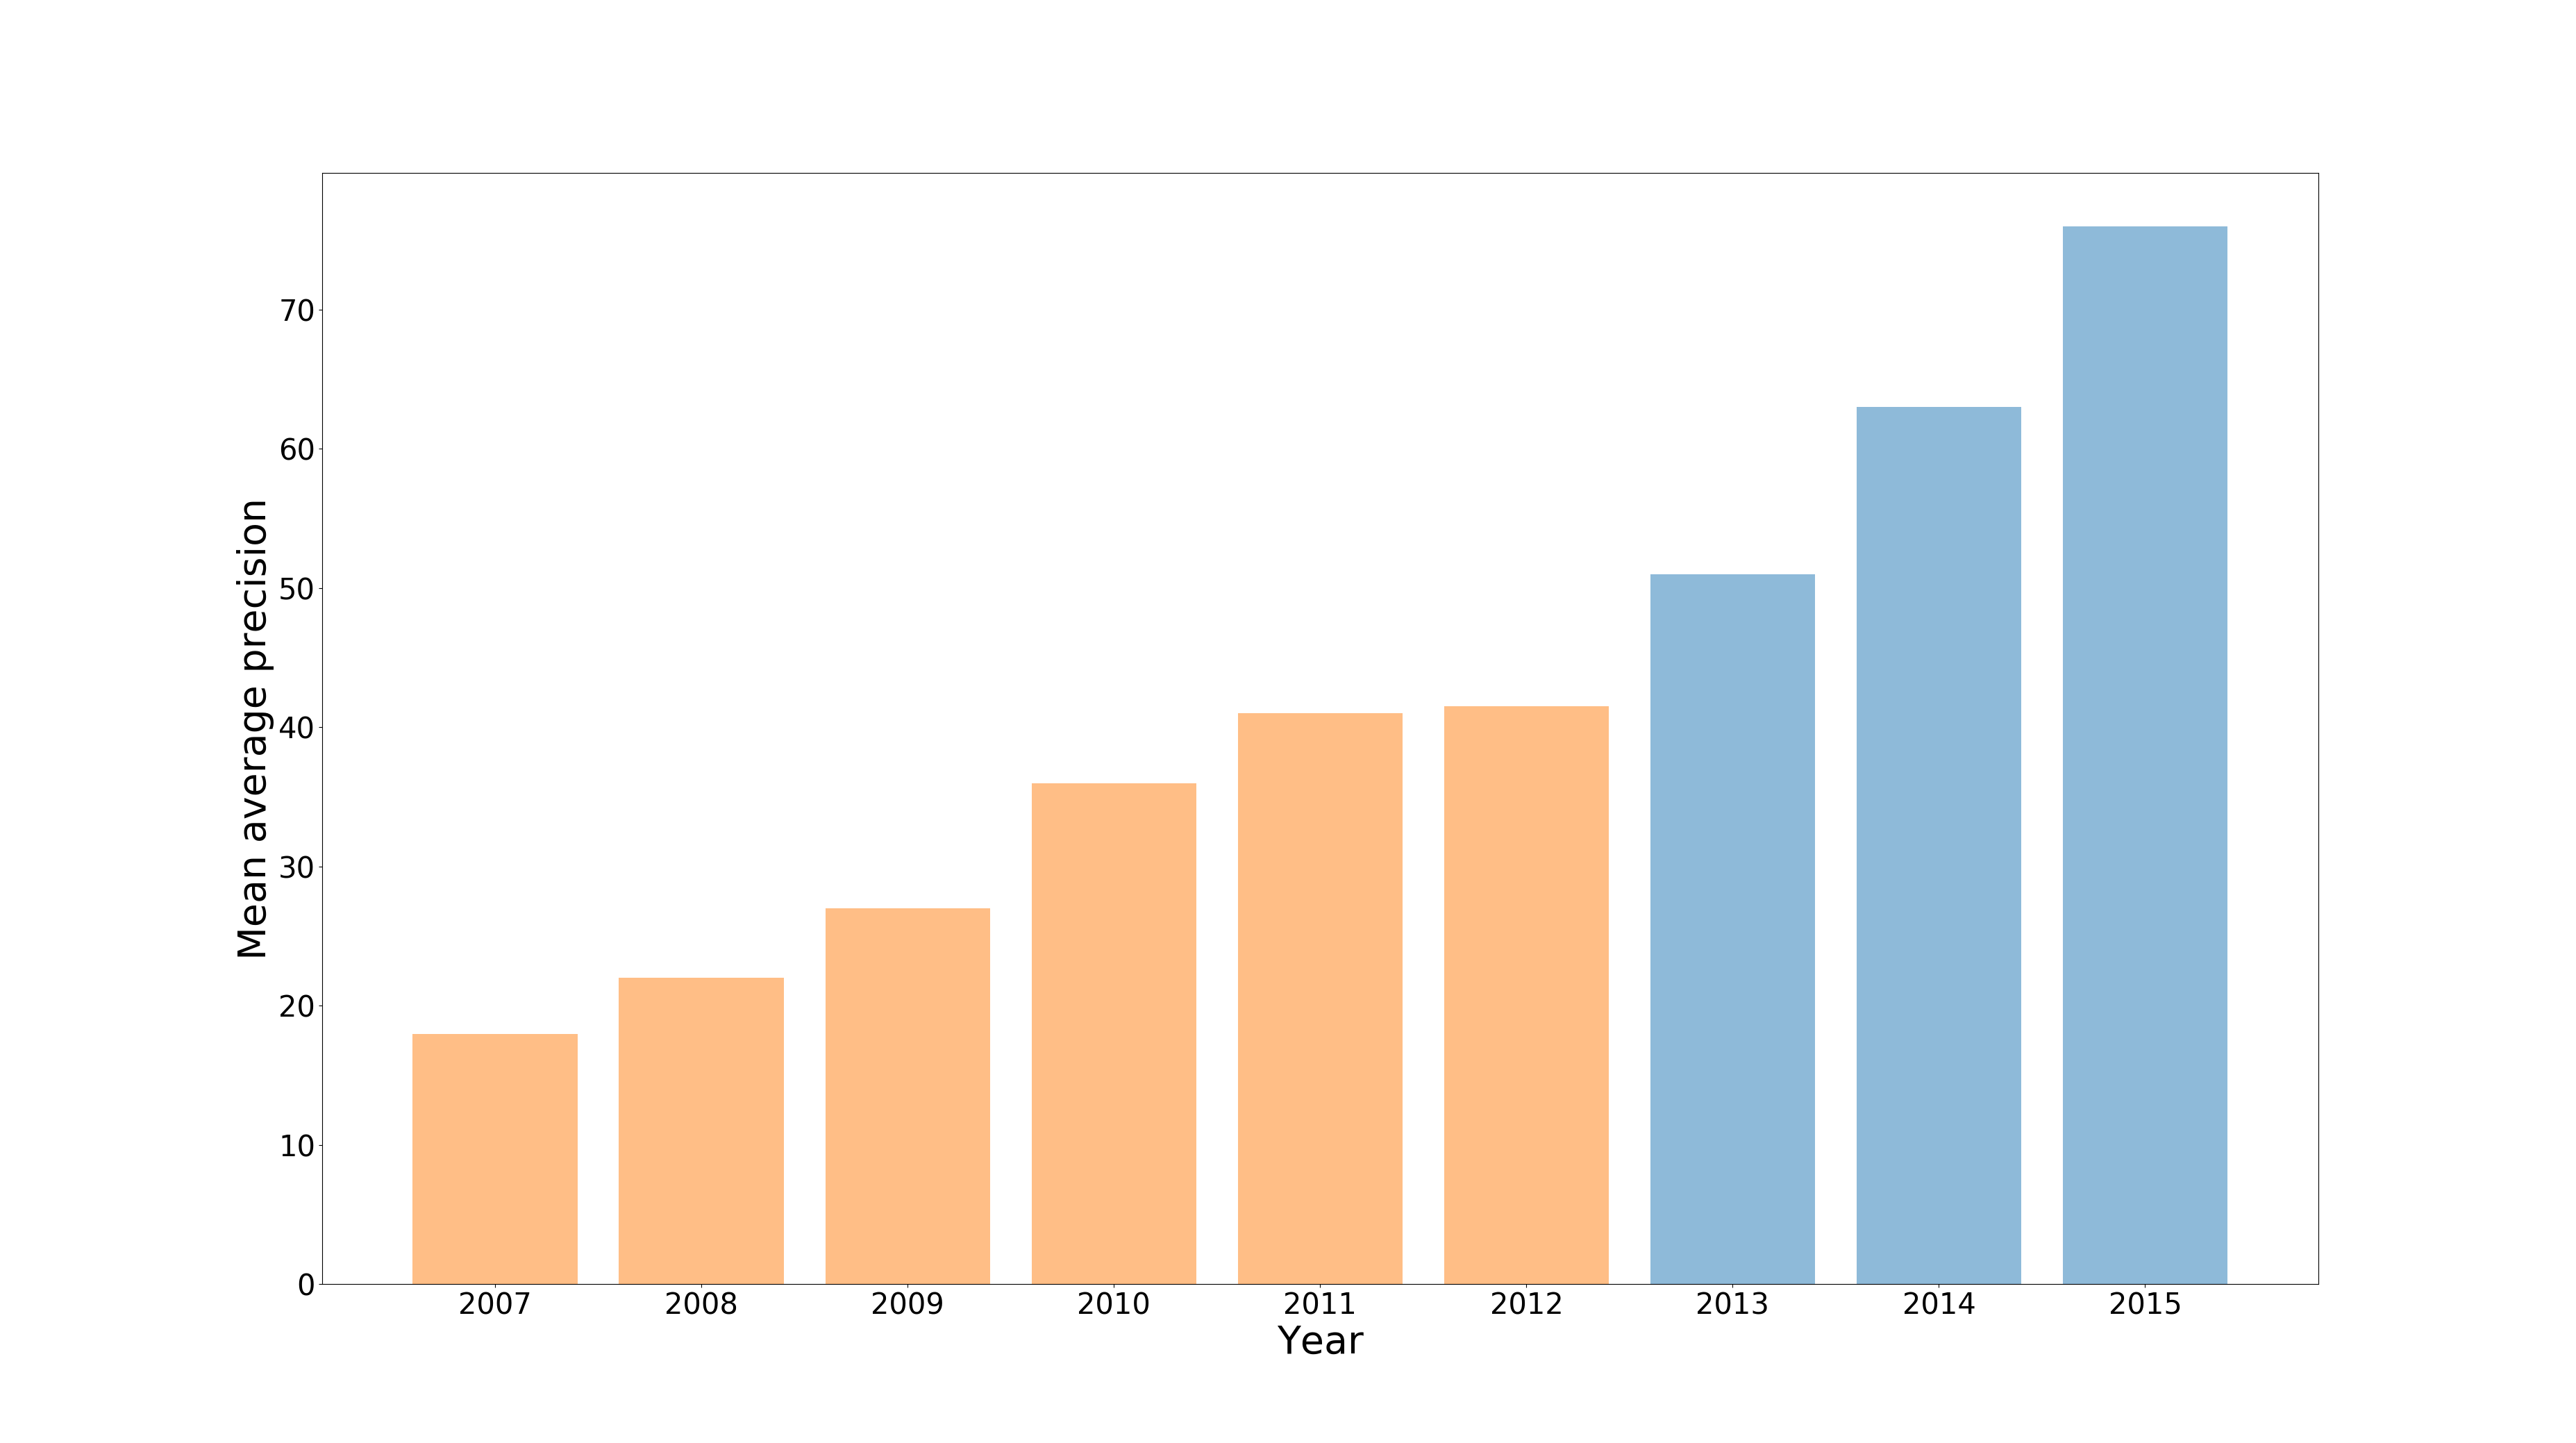
\includegraphics[width=0.7\linewidth]{intro/objesName.png}
\caption{Mean average precision over the years in PASCAL dataset.} \label{deepObjet}
\end{figure}


%Actual object detectors are based on three main family of architectures \cite{cnnComparision}, of which names are: FasterRCNN, RFCN, and SSD. In \ref{refArchite} we can observe a scheme of these systems.


Present deep learning object detectors are based on three main family of architectures \cite{cnnComparision}, named by the reference algorithm of the category: FasterRCNN, SSD, and RFCN, the characteristics of these systems are:

%\begin{figure}[H]
%		
%\centering
%
%\subfigure[Faster RCNN.]{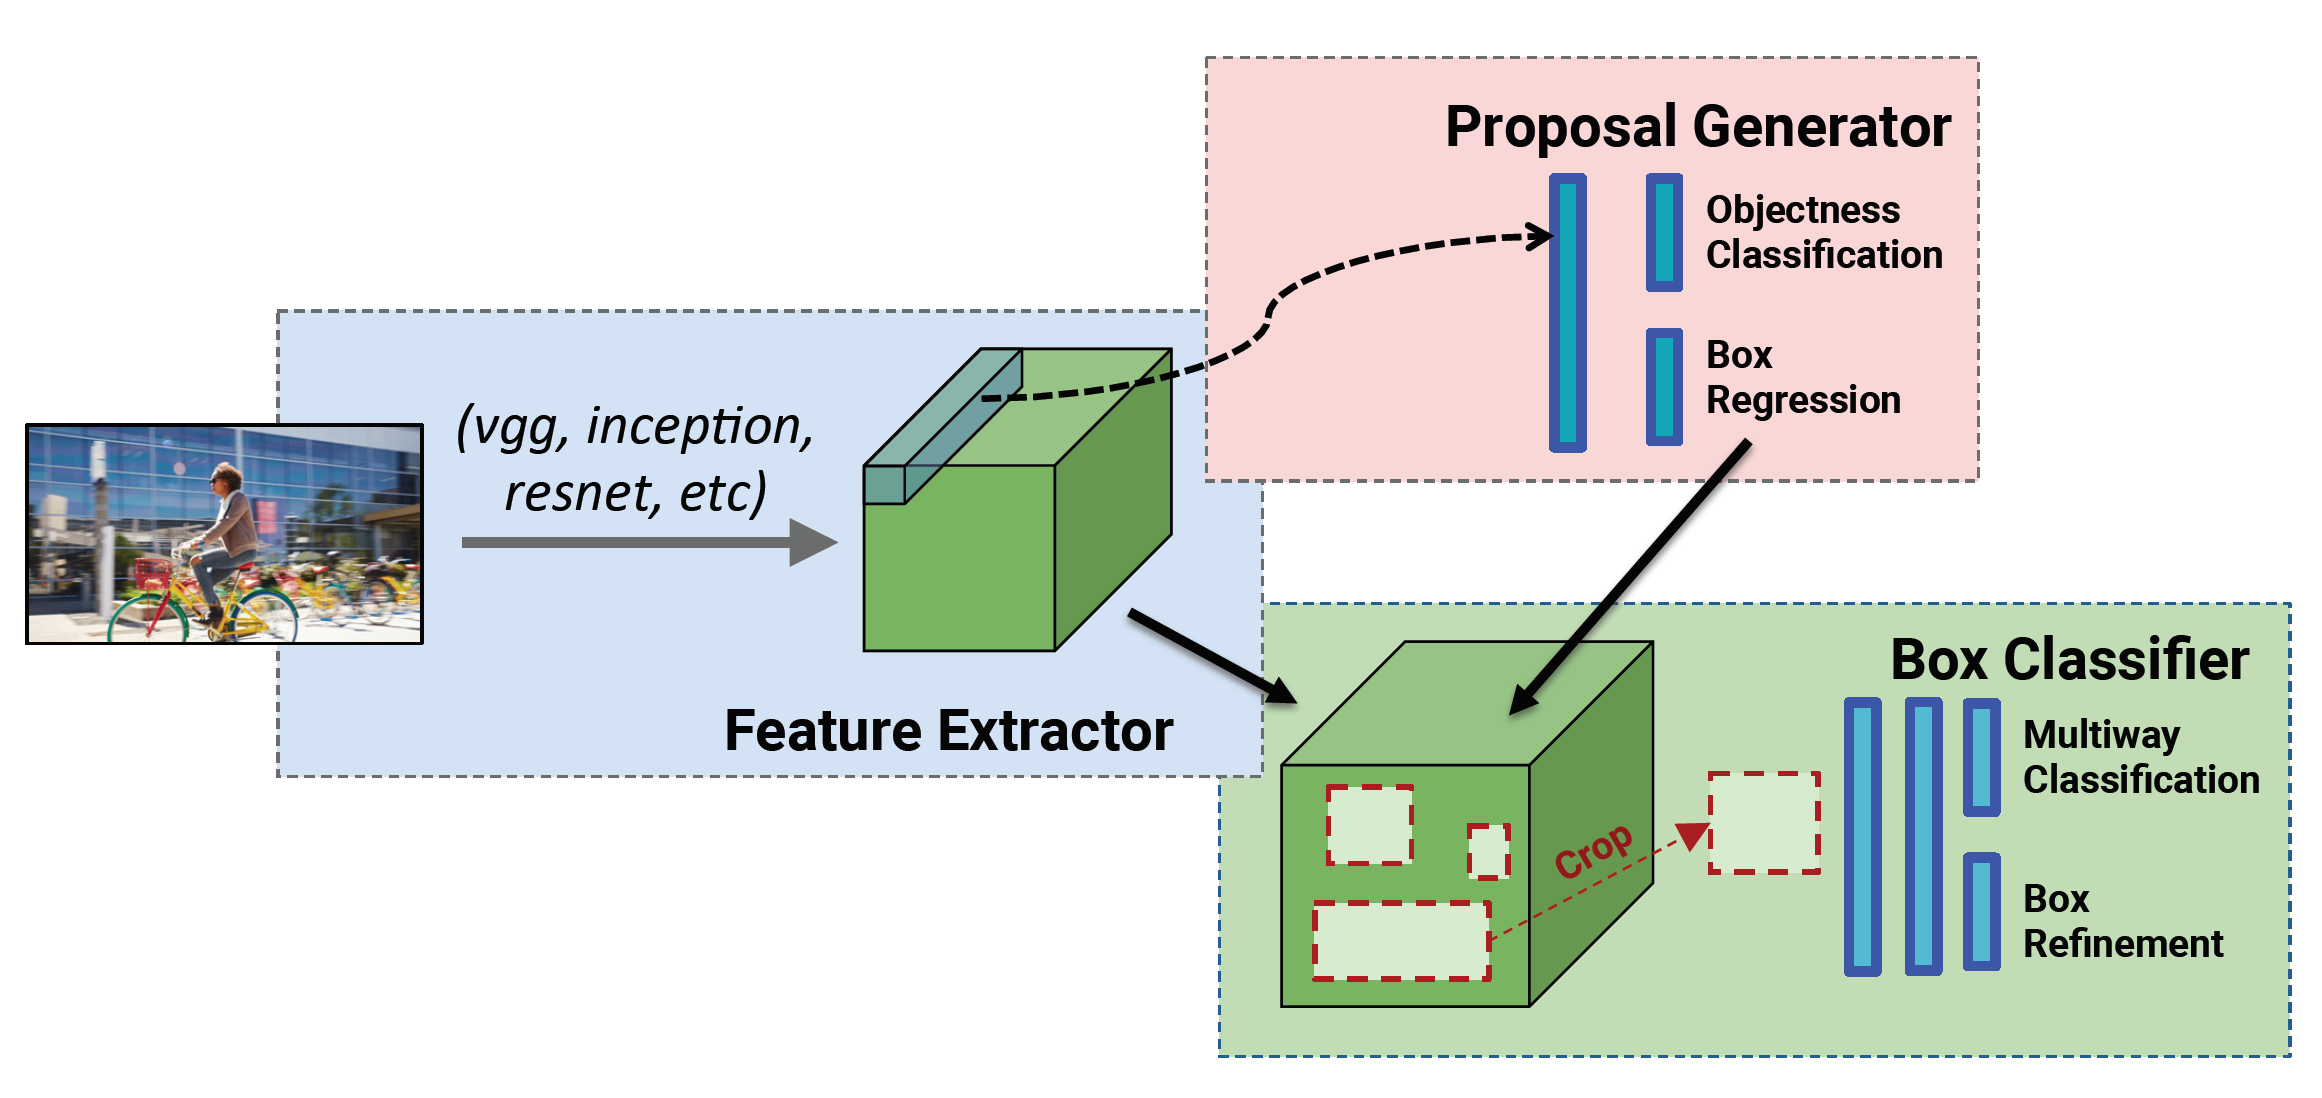
\includegraphics[width=5cm]{objectDetection/compFaster.png}}
%\subfigure[SSD.]{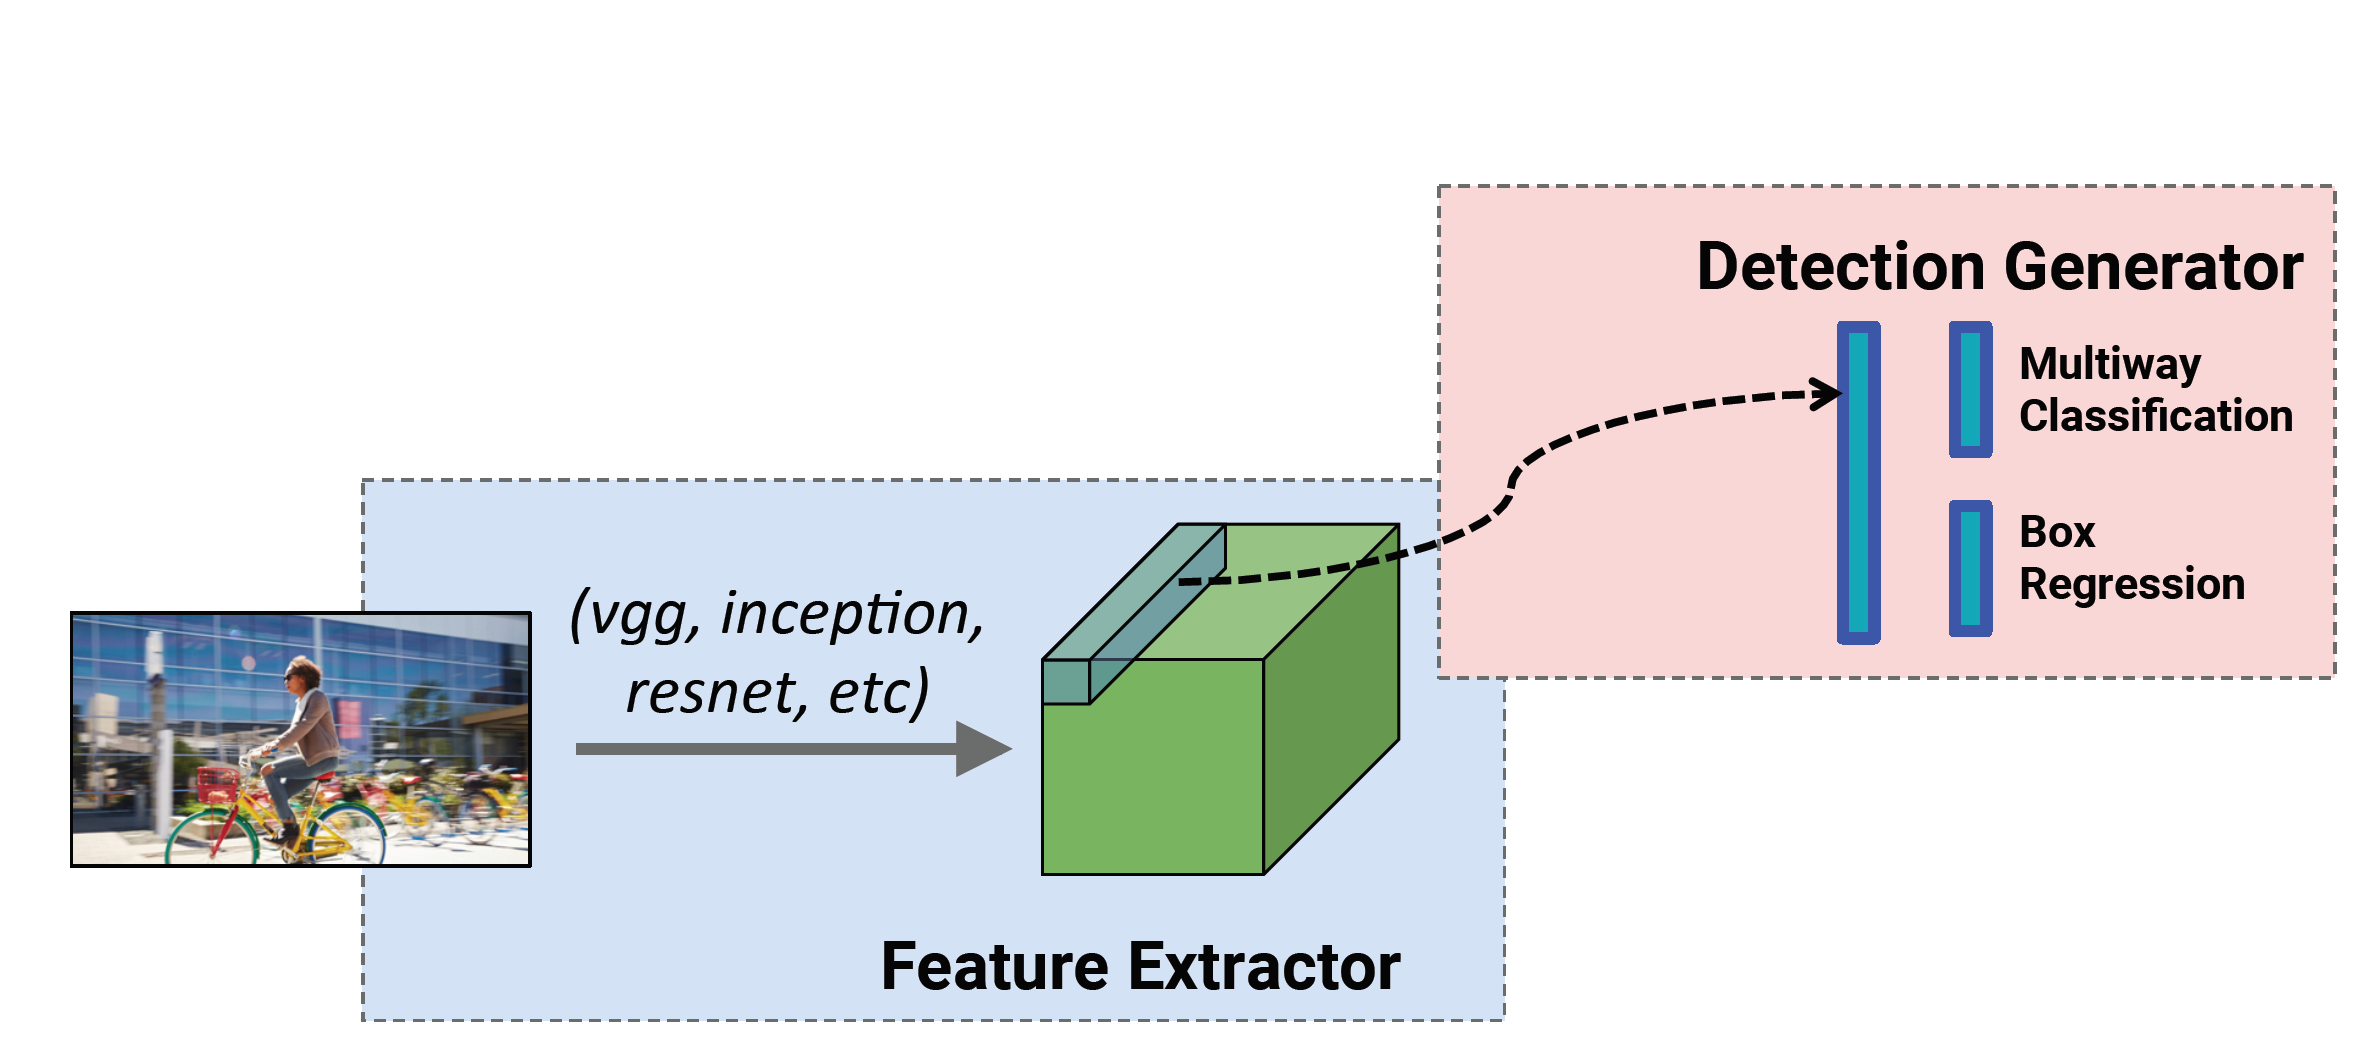
\includegraphics[width=5cm]{objectDetection/compSSD.png}}
%\subfigure[RFCN.]{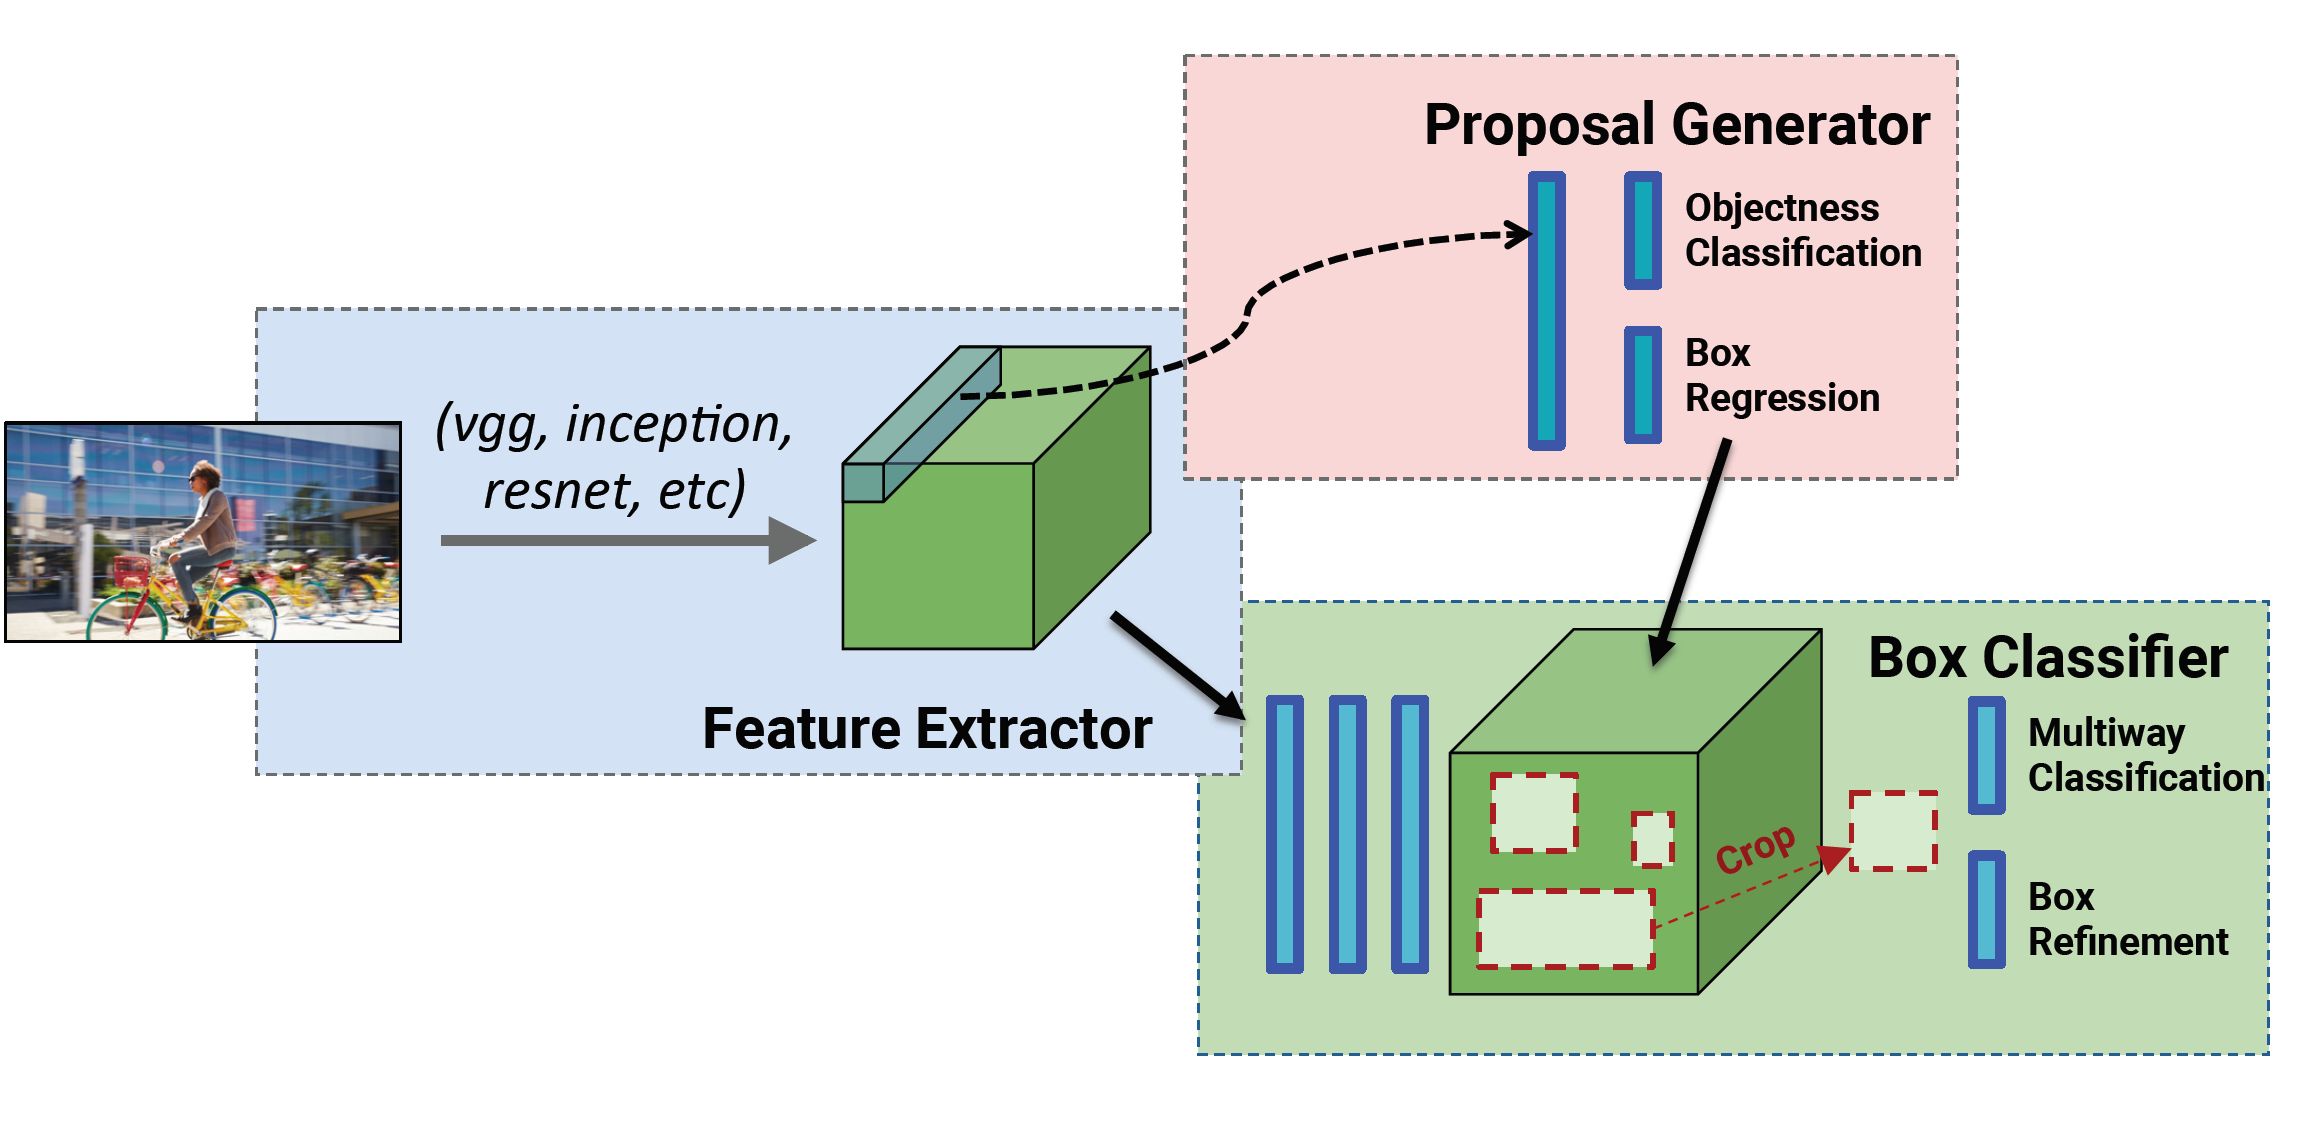
\includegraphics[width=5cm]{objectDetection/compRFCN.png}}\\
%
%\caption{Object detection architectures.}
%\label{refArchite}
%\end{figure}



\begin{itemize}

\item Faster RCNN \cite{fasterrcnn}, it is the last output of a trilogy of detectors developed by R. Girshick and his team. Which are called Region-Based object detectors. They work as follows: Use some mechanism to extract region of an image that are probable to be an object and then classify those proposals with a CNN. The first paper to do so, was \cite{rcnn}, and suppose a breakthrough in the field, increasing the precision of the state of the art of those days. But, it had a messy pipeline, slow and difficult to train. Later on, they developed \cite{fastrcnn}, in this paper they applied the region proposal algorithm in the cnn feature map, so, they avoid to compute the features for each proposal. They increase the speed and it could be trained much easily. Finally, they showed FasterRCNN \cite{fasterrcnn}, in this algorithm, they eluded the external region proposal algorithm and they implemented a CNN to compute those proposals. This CNN share parameters with the main net and they saved a lot of time. This network, has become the standard object detector with CNN. With the association of novel net architecture like ResNet \cite{resnet}, Inception \cite{inception}, and \cite{pvanet} they have won all the contests.


\item SSD, it stands for Single shot multibox detector. These family of method differs from previous ones considering that these treats the problem of object detection as a regression problem. So, they are called Regression-based object detector or single shot object detector due it does not have a region proposal algorithm, they classify the image with one mechanism. The maximum exponent of these algorithms are \cite{yolo} and \cite{ssd}. These work as follows, they discretize the image at the features level in a fixed grid and for each grid it predicts a class and some number of bounding boxes with different shapes and sizes. It merges all, and apply a Non-Maximum suppression algorithm to obtain a set of detections. We can observe this process in \ref{yolo1}. In addition, they apply this process in a multiresolution scheme as we can observe in \ref{yolo2} to deal with objects of different sizes.

\begin{figure}[H]
		
\centering

\subfigure[Input Image.]{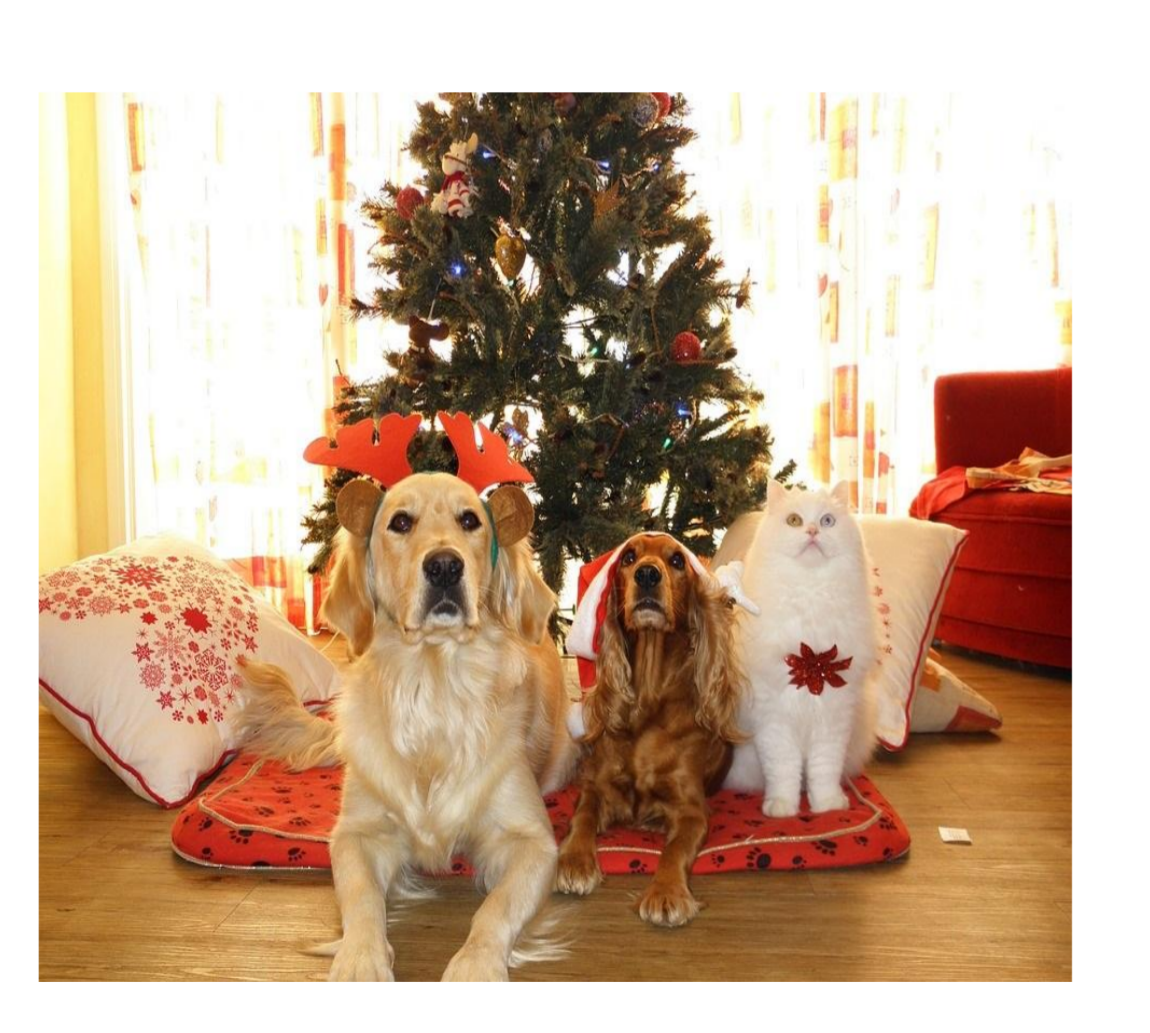
\includegraphics[width=7cm]{objectDetection/retall1.png}}
\subfigure[Divide image into grid.]{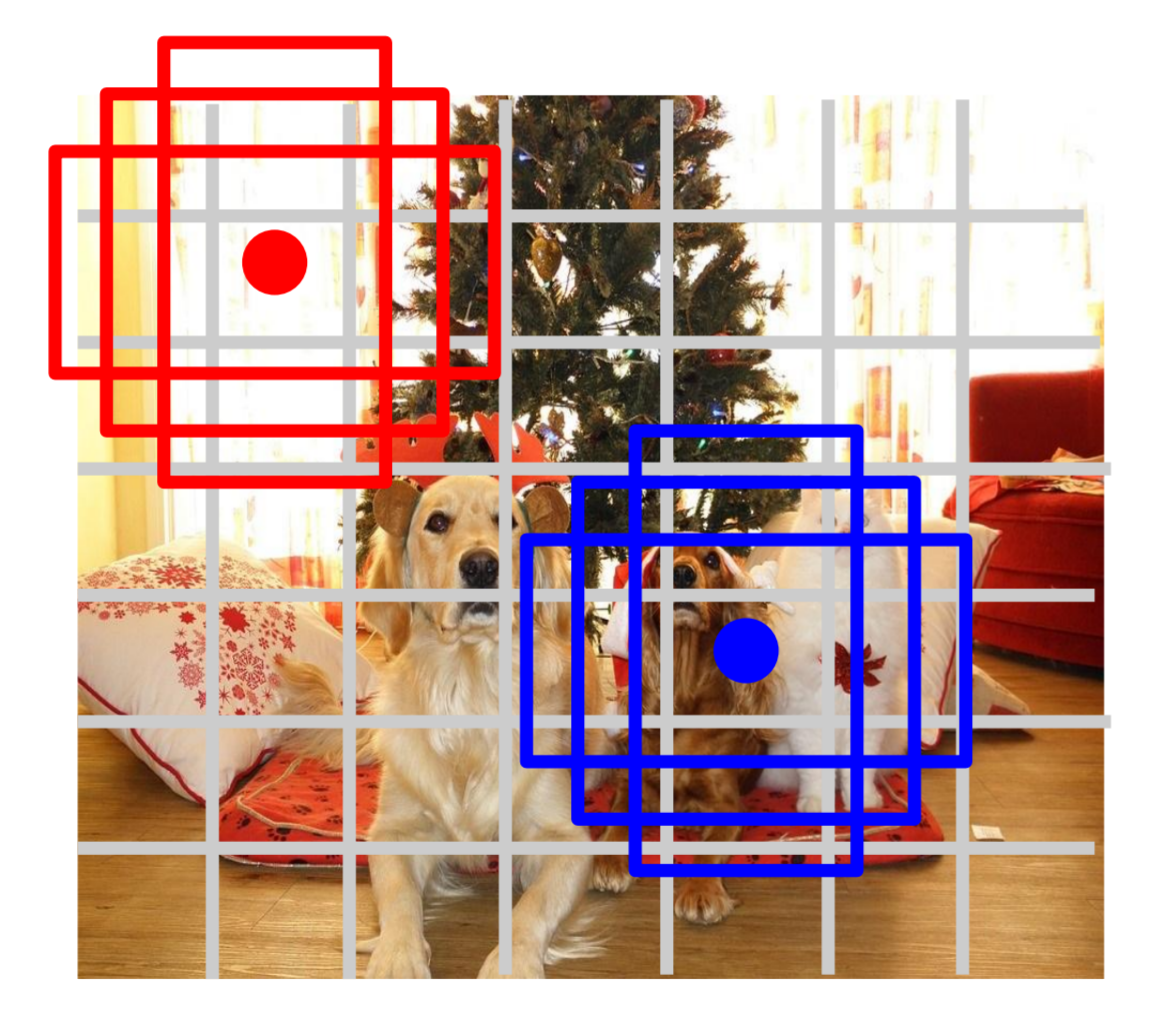
\includegraphics[width=7cm]{objectDetection/retall2.png}}\\


\caption{SSD detector scheme.}
\label{yolo1}
\end{figure}


\begin{figure}[H]
\centering         
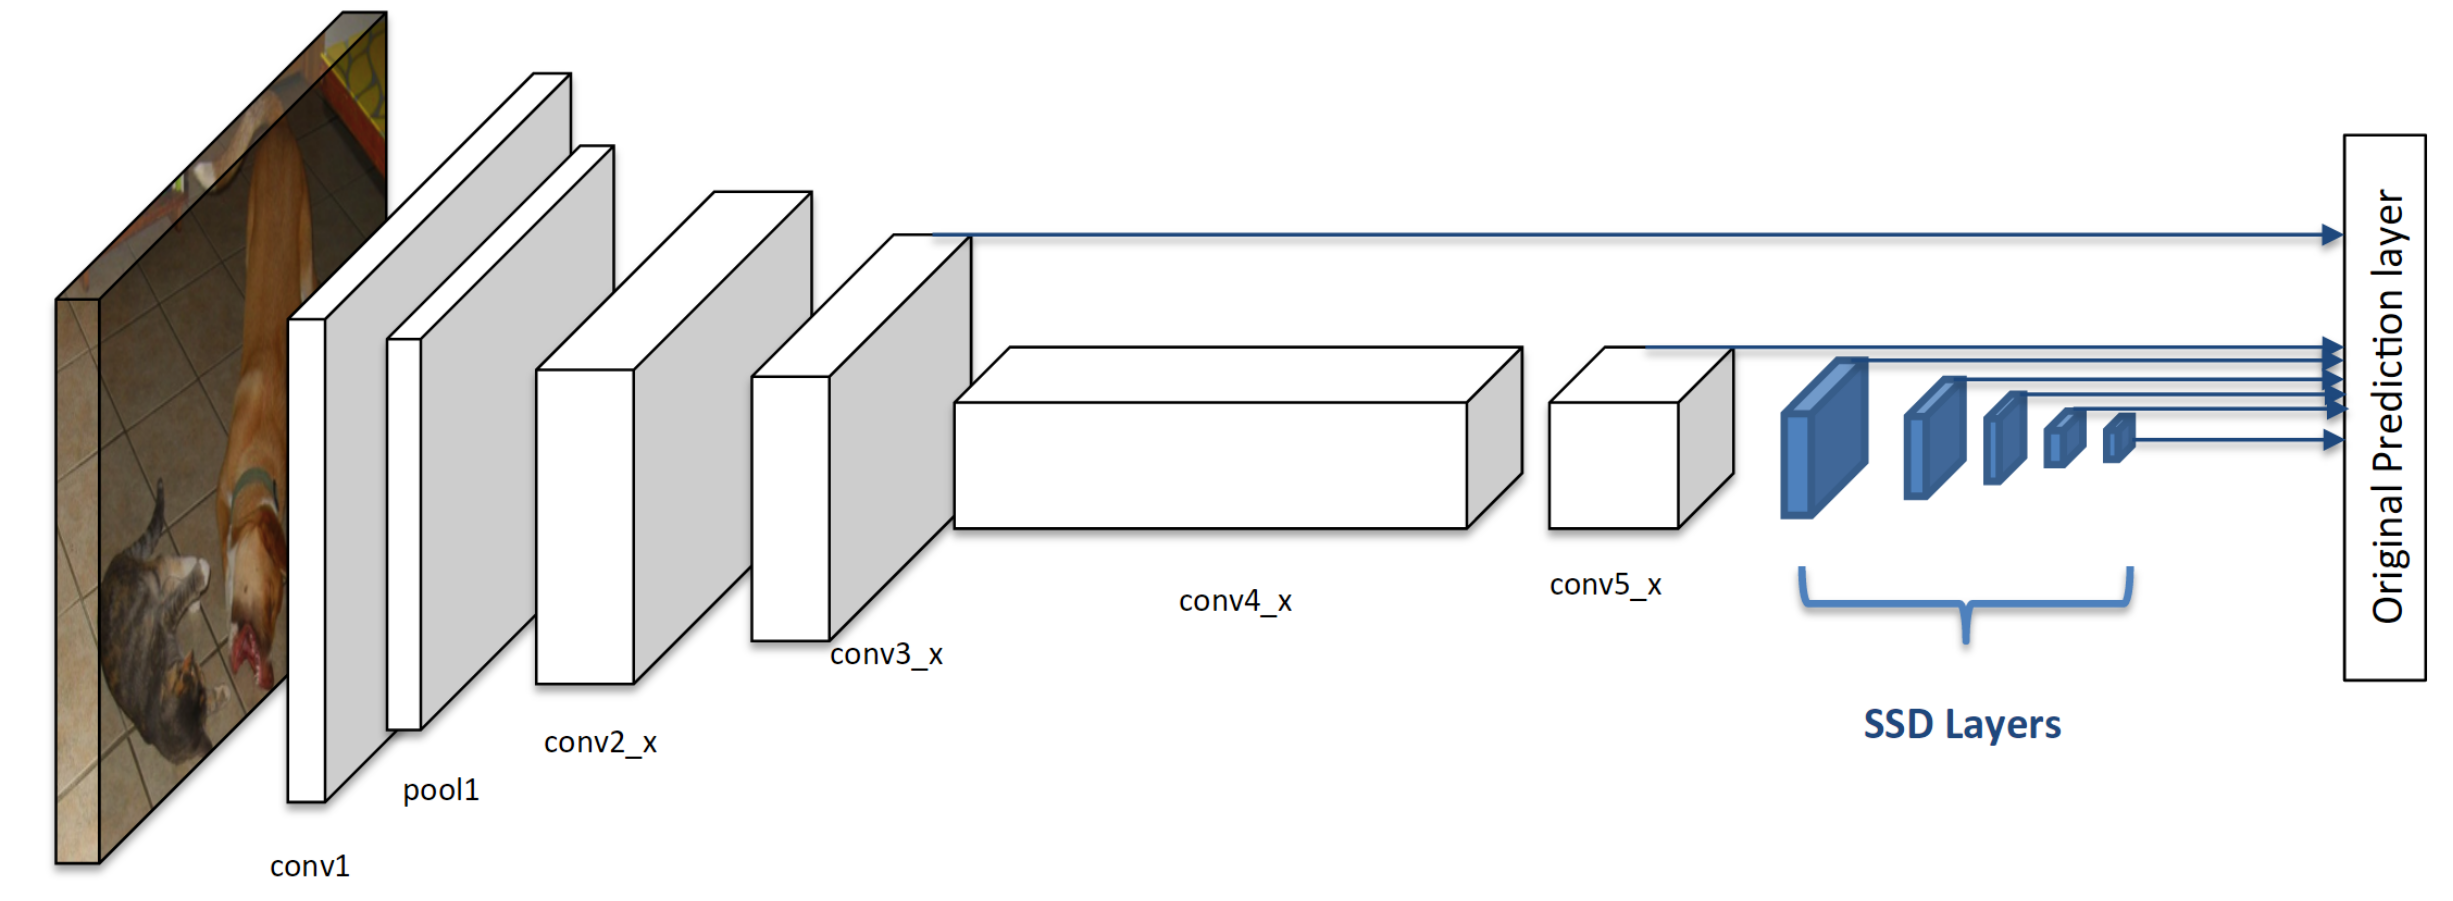
\includegraphics[width=12cm]{objectDetection/ssdArchitecture2.png}
\caption{SSD architecture.} \label{yolo2}
\end{figure}



\item RFCN \cite{rfcn}, it stands for Region-based fully convolutional network and it was developed by the same authors of SSD. They noticed the lacks of the SSD, the SSD algorithm computes the object detector on the feature map, and at this level the features have a low spatial resolution, this involves do not detect small objects. So the authors inspired by the fully convolutional architectures, upsample those feature maps and compute the object detector like the SSD algorithm.

\end{itemize}



In the survey \cite{cnnComparision}, they compared the different methods including changing the features extractors ( ResNet, Inception, VGG ) and they measured the precision ( mean average precision ) and computing time. This results are showed in \ref{comparisio}. The conclusion are as follows, SSD is the fastest detector, RFCN it has the best balance between speed-accuracy, and FasterRCNN, is the most accurate detector although is slower than the other ones.



\begin{figure}[H]
\centering         
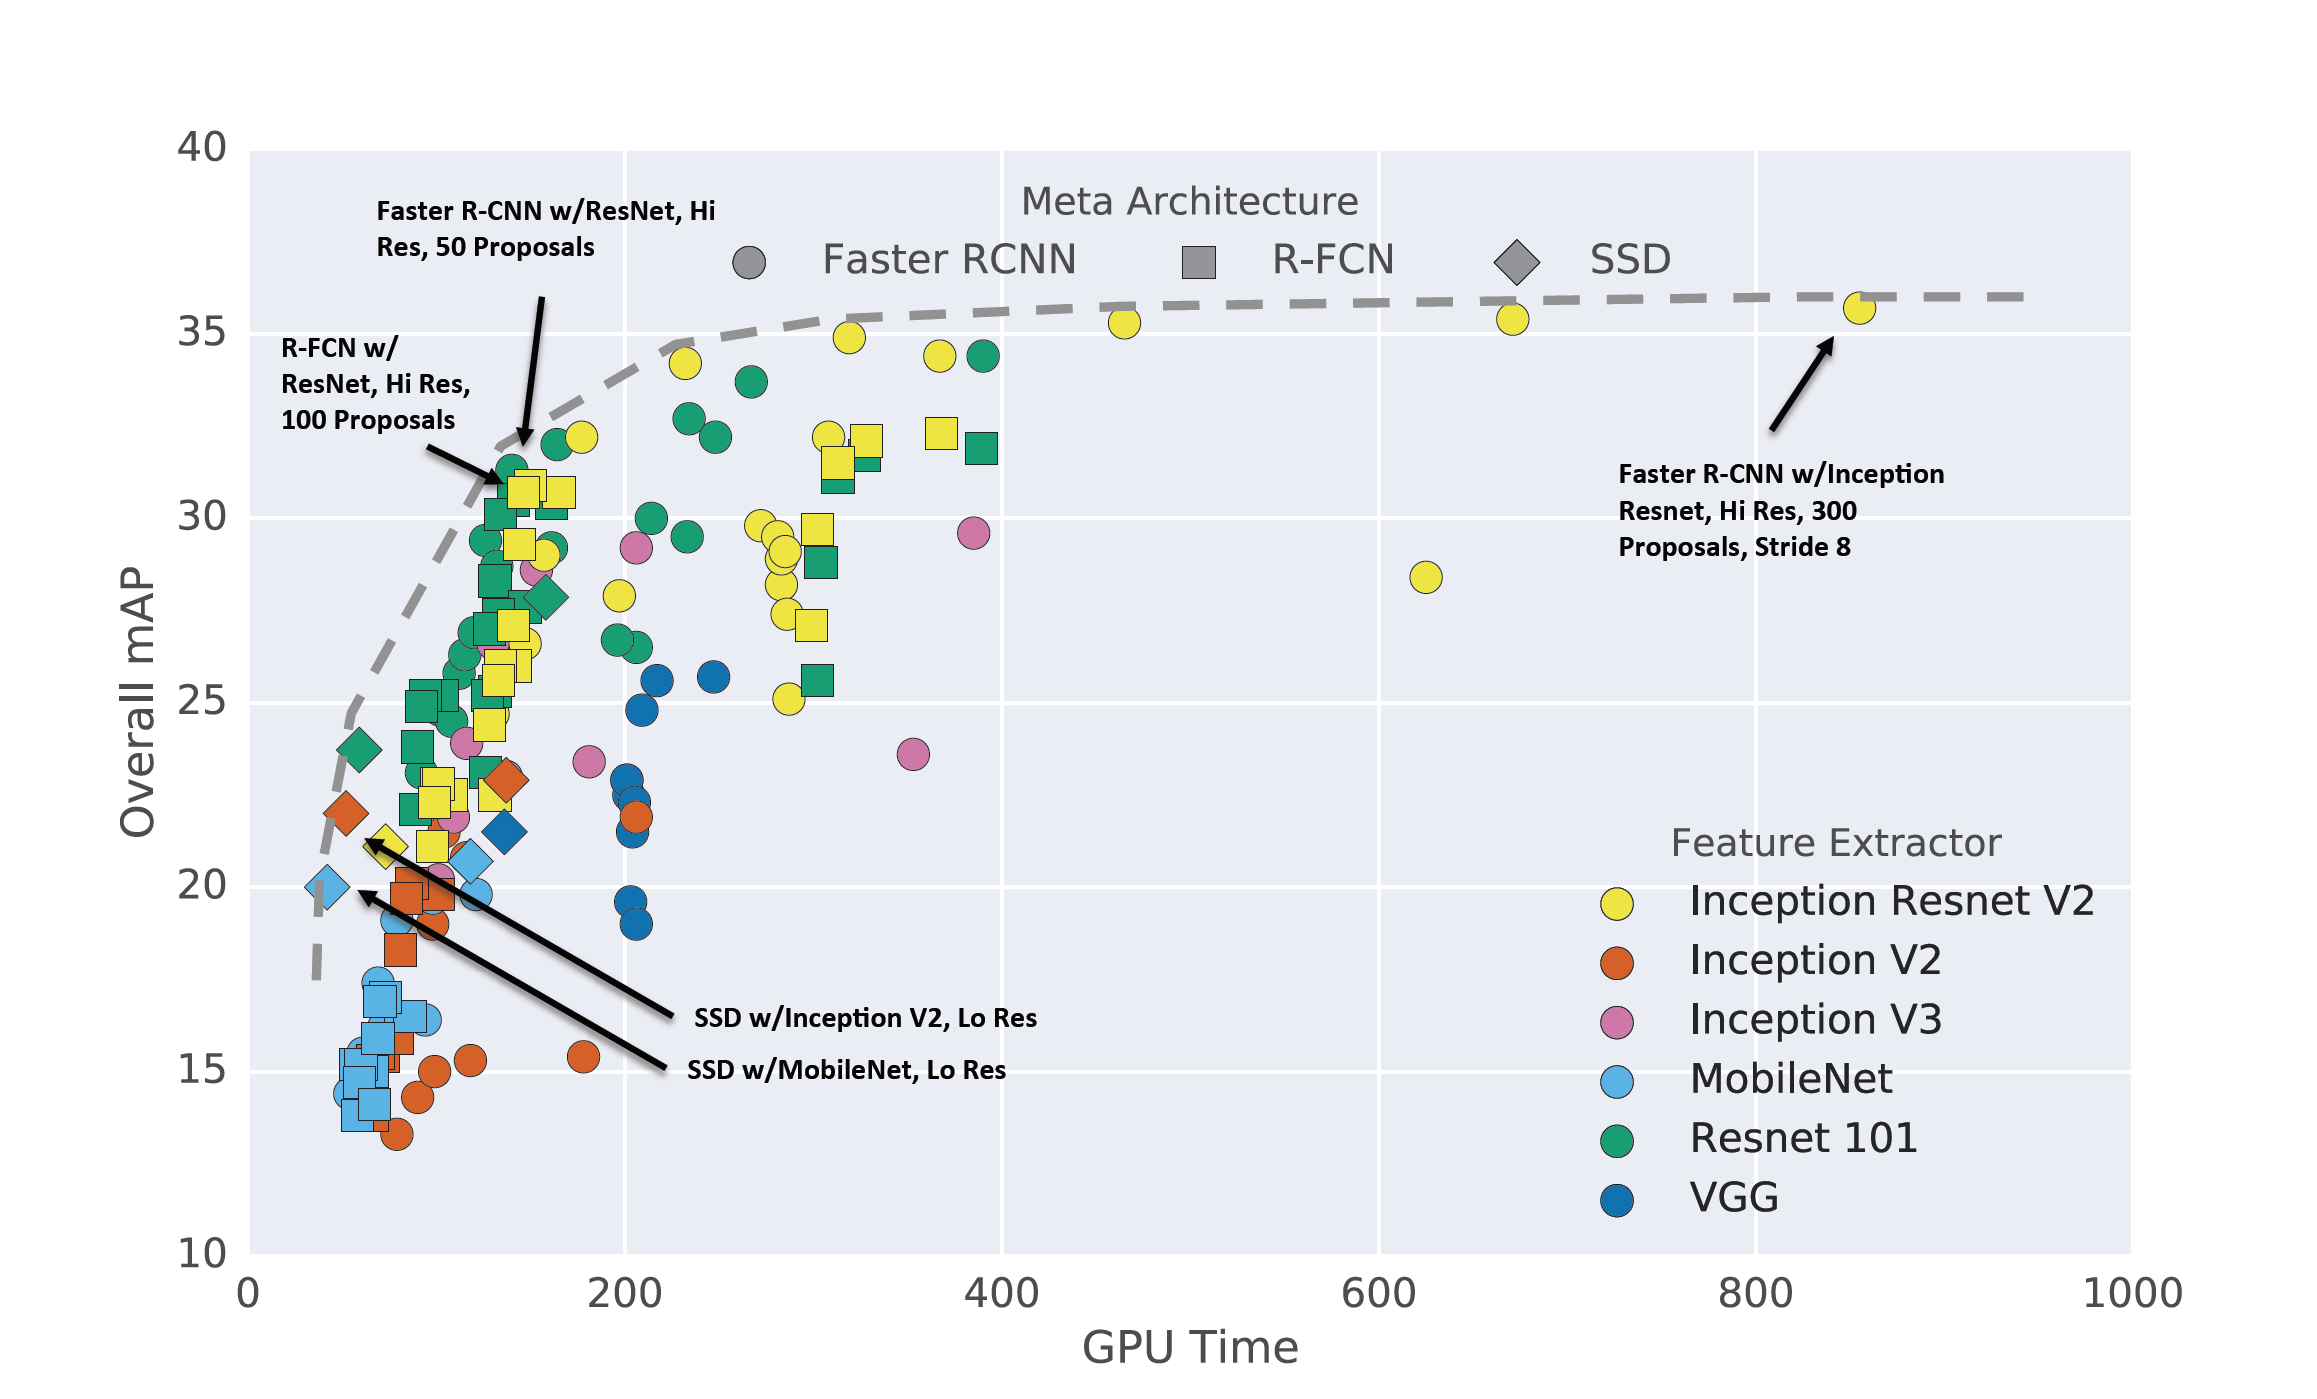
\includegraphics[width=0.9\linewidth]{objectDetection/comparisionTensor.png}
\caption{Comparison architectures.} \label{comparisio}
\end{figure}

We will finish off our review with a numeric comparison of the methods, as we can observe in the table \ref{tableDet}. This information is extracted from the original papers with their implementation, all of them are trained with the union of the training set of VOC07, VOC12, and COCO, and subsequently evaluate on VOC07 test set on a Nvidia Titan X GPU. These results give us an intuition on which detector will be suitable for our task.

\begin{table}[H]
\centering

\begin{tabular}{lllll}
                    & \textbf{mAP} & \textbf{mAP\_person} & \textbf{FPS} & \textbf{Proposals} \\
\textit{RCNN}       & 66           & 64.2                 & 0.077        & 2000               \\
\textit{FastRCNN}   & 70           & 69.9                 & 6.7          & 2000               \\
\textit{FasterRCNN} & 85.6         & 82.3                 & 7            & 6000               \\
\textit{SSD300}     & 81.2         & 81.4                 & 46           & 8732               \\
\textit{SSD512}     & 83.2         & 84.6                 & 19           & 24564              \\
\textit{YOLO}       & 66.4         & 63.5                 & 45           & 98                 \\
\textit{YOLOv2}     & 78.6         & 81.3                 & 40           & -                  \\
\textit{RFCN}       & 83.6         & -                    & 10           & -                  \\
\textit{PVANET}     & 84.9         & -                    & 31.3         & 300               
\end{tabular}

\caption{Summarize of the object detectors.}
\label{tableDet}
\end{table}


\subsubsection{Feature tracking}


\subsubsection{Features}\label{feature}

Our goal is to find points in an image, that can be found in other images and then compute some information, in this case, the movement. The characteristics of good features are:

\begin{itemize}

\item Repeatability, the same feature can be found in several images despite geometric and photometric transformations.

\item Matchability, each feature has a distinctive description, thus easy to find.

\item Efficiency, few features have to compact much more possible information.

\item Locality, a feature occupies a relatively small area of the image, so therefore it is robust to clutter and occlusion.

\item Performance, computation speed of features is a critical parameter. 

\end{itemize}

Features points are used in all sort of operations in computer vision: Image alignment, 3D reconstruction, Motion Tracking, Object recognition, Index database retrieval, robot navigation and so on.

Looking at the figure \ref{patches}, the flat patch, is a patch without texture and impossible to localize. Patches with large contrast edges are easier to localize, although straight lines segments at a single orientation suffer from the \textit{aperture problem}, are also impossible to localize. Finally, patches with large gradients in at least two different orientations are the easiest to localize.

\begin{figure}[H]
		
\centering

\subfigure[Flat region.]{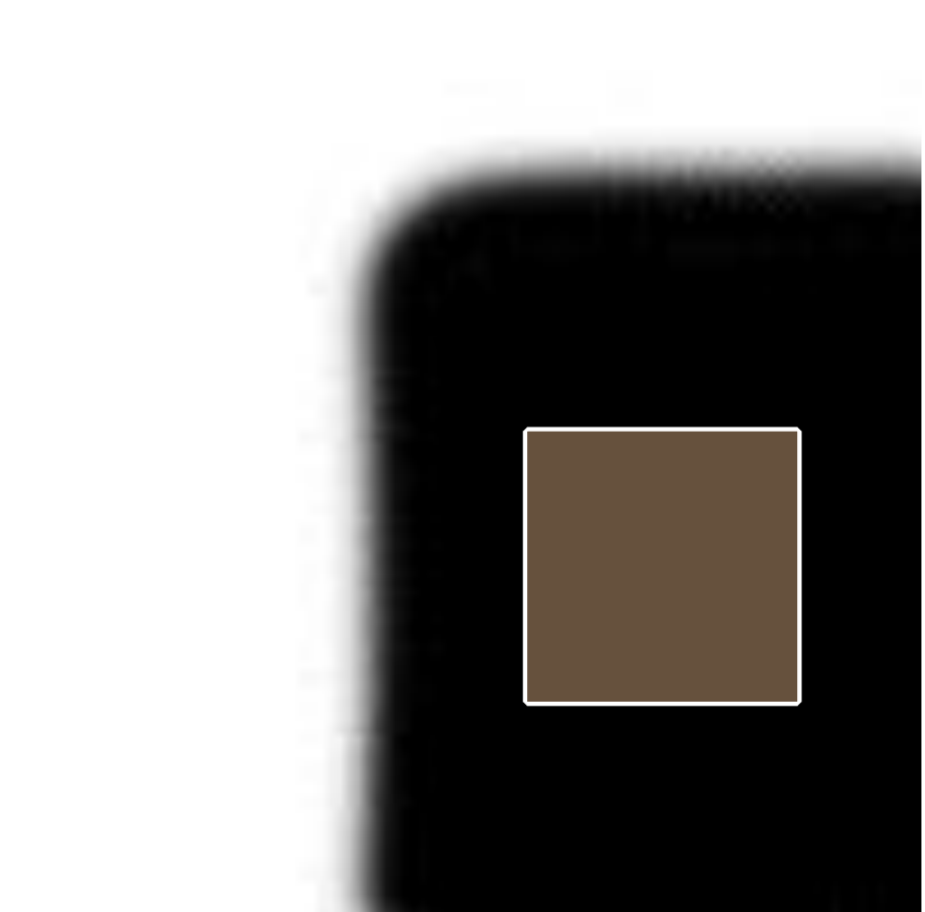
\includegraphics[width=5cm]{lucasKanade/flat.png}}
\subfigure[Edge region.]{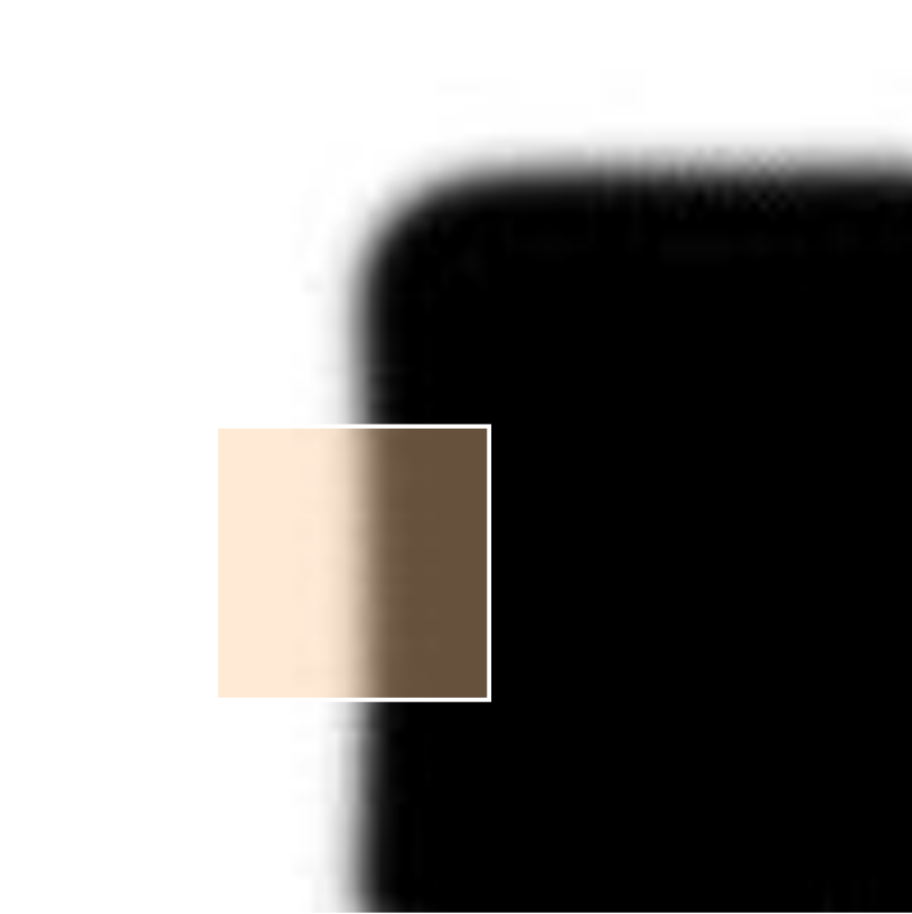
\includegraphics[width=5cm]{lucasKanade/edge.png}}
\subfigure[Corner region.]{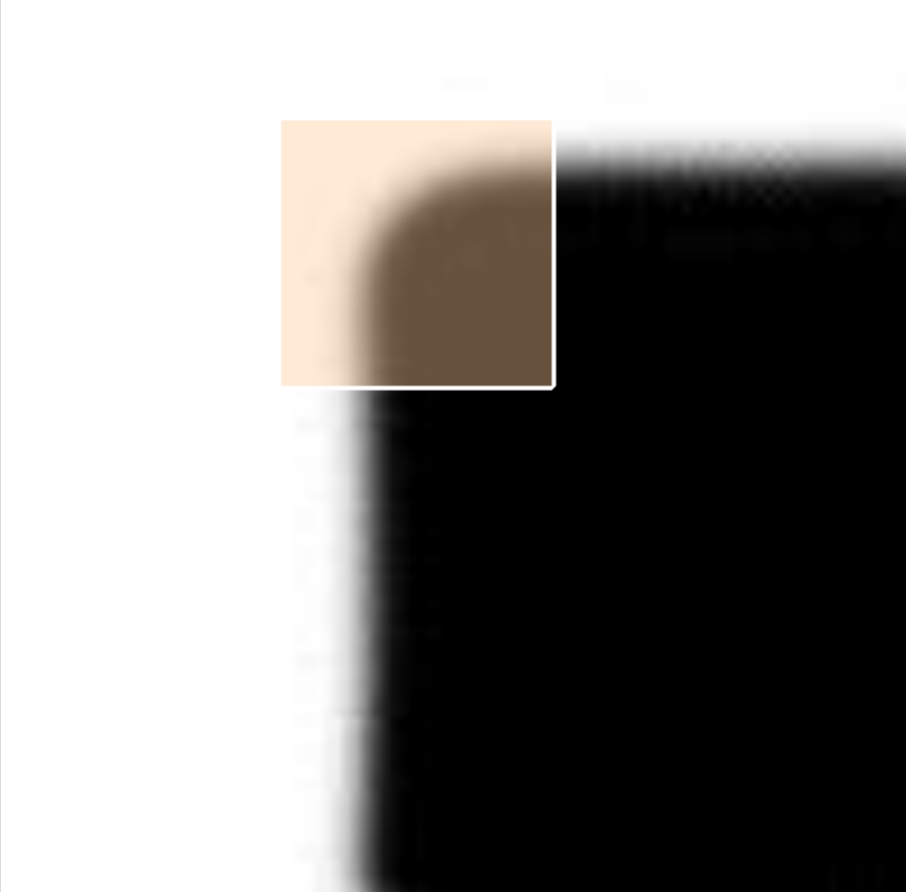
\includegraphics[width=5cm]{lucasKanade/corner.png}}\\


\caption{Types of patches.}
\label{patches}
\end{figure}

These intuitions can be formalized by looking at the simples possible matching criterion for comparing two images patches, their weighted summed square difference:

%Change in appearance for the shift [u,v]:

%$$ E(u,v) = \sum_{x,y} w(x,y) [I(x+u,y+v)-I(x,y)]^{2}$$
$$ E(u) = \sum_{i} w(x_{i}) [I(x_{i}+u)-I(x_{i})]^{2}$$

where $I(x)$ is the image, $I(x+u)$ is the shifted image, and $w(x,y)$ is a window function like a box or gaussian kernel around the pixel, and the summation $i$ is over all the pixels in the patch. Then we are looking for points, which if we move according to $u$ we have a change. 



When performing feature detection, we do not know which other image locations the feature will end up being matched against. Therefore, we can only compute how stable this metric is with respect to small variations in positions $\Delta u$ by comparing an image patch against itself:

$$ E( \Delta u) = \sum_{i} w(x_{i}) [I(x_{i}+\Delta u)-I(x_{i})]^{2}$$

Using a Taylor series expansion of the image function $I(x_{i}+\Delta u) \approx I(x_{i}) + \nabla I(x_{i})*\Delta u  $ we can approximate the expression as follows:

$$ E( \Delta u) \approx \sum_{i} w(x_{i}) [I(x_{i})+\nabla I(x_{i}) \Delta u-I(x_{i})]^{2}$$


$$ E( \Delta u) = \sum_{i} w(x_{i}) [\nabla I(x_{i}) \Delta u]^{2}$$

With algebraic notation it transforms to:

$$ E( \Delta u) = \Delta u^{T} M \Delta u$$

where $ \nabla I(x_{i}) = [I_{x},I_{y}](x_{i}) $ is the image gradient and $M$ is the second moment matrix:

\[ M = \left( \begin{array}{ccc}
I_{x}^{2} & I_{xy}^{2} \\
I_{xy}^{2} & I_{y}^{2} \end{array} \right).\] 

Computing the eigenvalue decomposition of this matrix, shows the directions of the fastest change, thus a measure of the \textit{cornernes}. There are several algorithms that use in different ways this eigenvalues:

%In the figure \ref{corner} we can observe the relationship between eigenvalues and patches types.
%
%
%
%
%\begin{figure}[H]
%\centering         
%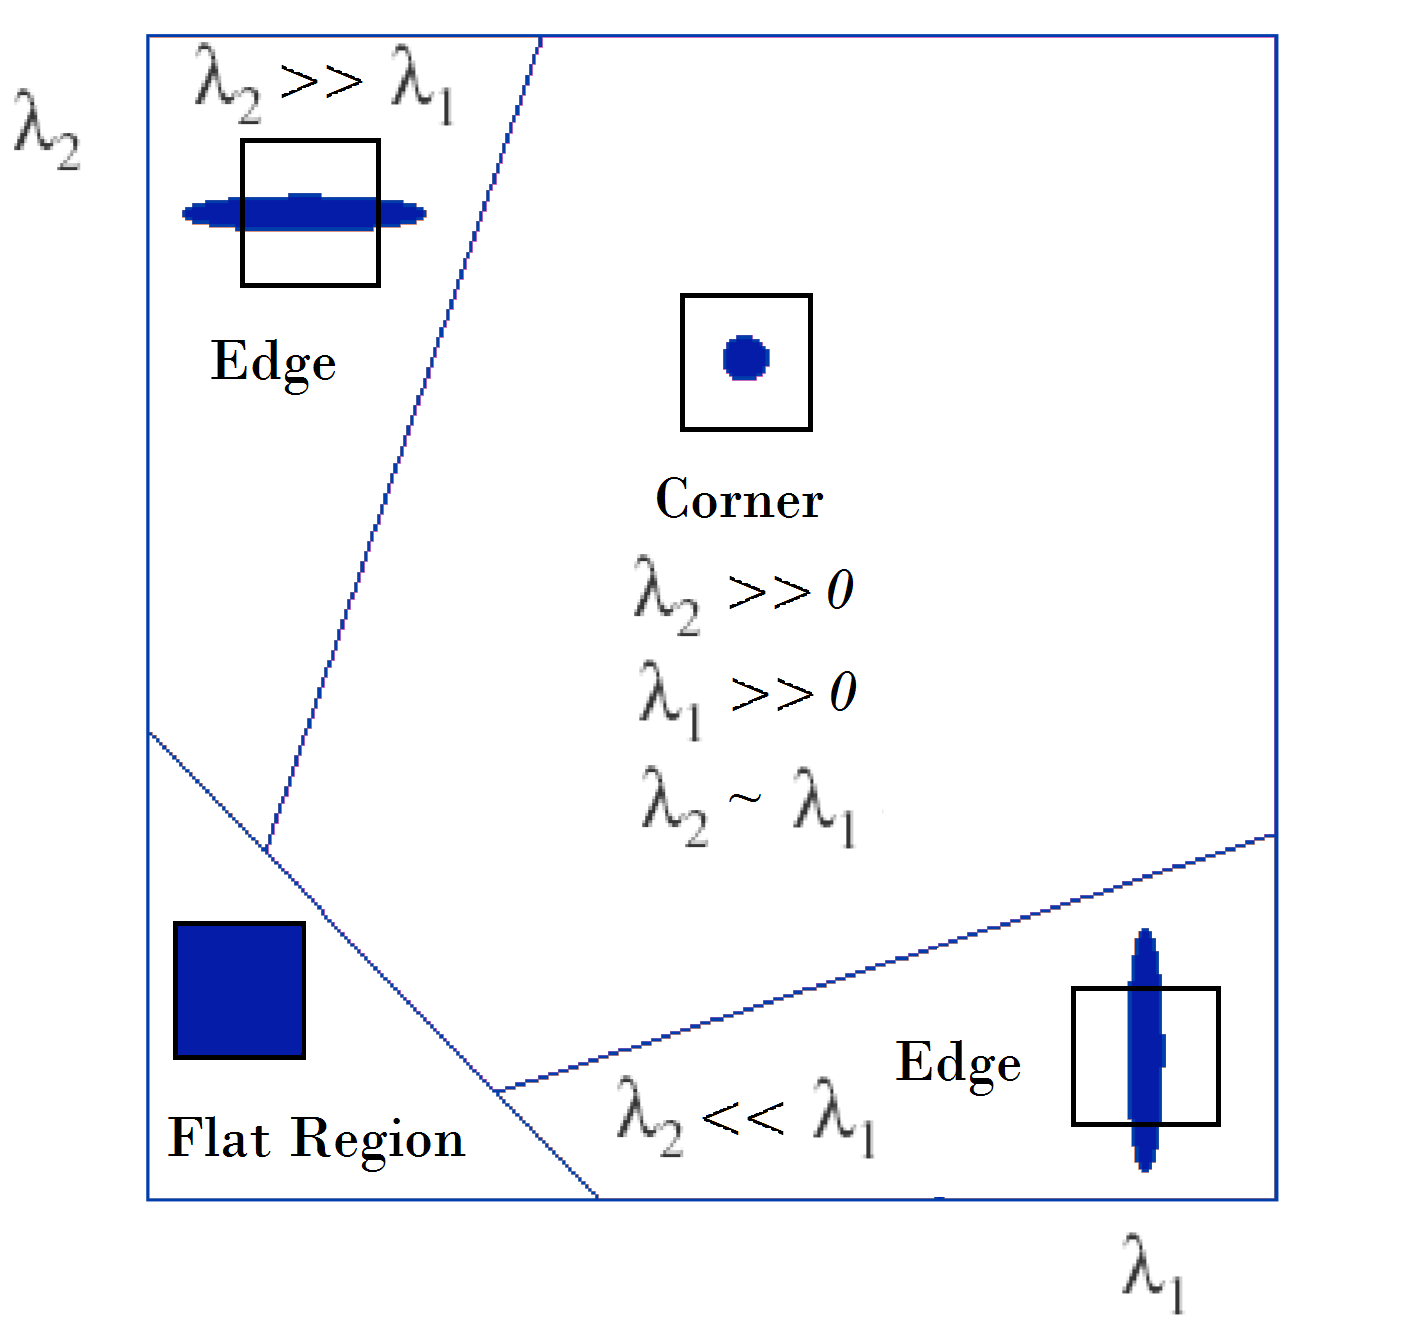
\includegraphics[width=0.6\linewidth]{lucasKanade/harrisMillora.png}
%\caption{Eigenvalues response for different regions .} \label{corner}
%\end{figure}




%There are several algorithms that use in different ways this eigenvalues:

\begin{itemize}

\item Harris \cite{harris}, they propose a corner detection response function. So for each pixel, they compute a matrix $M$ and with it, they compute the function
R, $R = det(M)-a \hspace{0.1cm} trace^{2}(M)$. if R is large, that pixel is a corner, if R is negative with larger magnitude, it is a an edge, and if R is small it is a 
flat region. So the they a threshold to classify those pixels as a corner. 

\item Shi-Tomasi \cite{shi}, they define the \textit{cornerness} in another way. The image has a maximum value ( e.g. 255), so $\lambda_{1}$, $\lambda_{2}$ also have an upper bound, then it is only necessary to check that $min(\lambda_{1},\lambda_{2})$ is large enough, this is how they define \textit{cornerness}. This feature is called good features to track, because the authors defined a \textit{good} features those whose motion can be estimated reliably, and they reached the same conclusions as Harris. This method is implement in the OpenCV's routine \texttt{goodFeaturesToTrack()}.

\end{itemize}

\subsubsection{Motion estimation}

Now, we have invariant points, we want to estimate the motion of those points. In order to do so, we compute the optical flow. This is the apparent two-dimensional motion of brightness pattern in the image. In the next figure \ref{refArchiteOF} we visualized this idea.


\begin{figure}[H]
		
\centering

\subfigure[$I(x,y,t) $.]{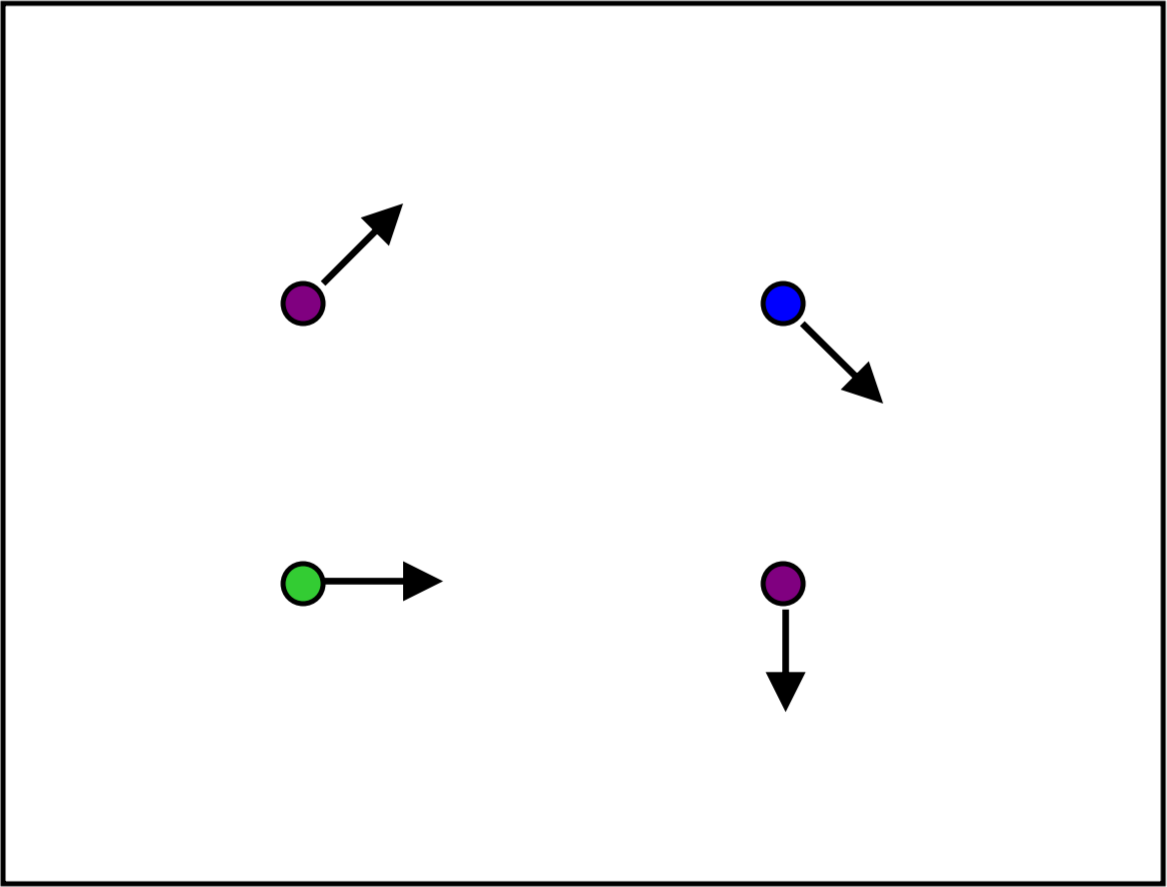
\includegraphics[width=5cm]{lucasKanade/retall1g.png}}
\subfigure[$I(x,y,t+1) $.]{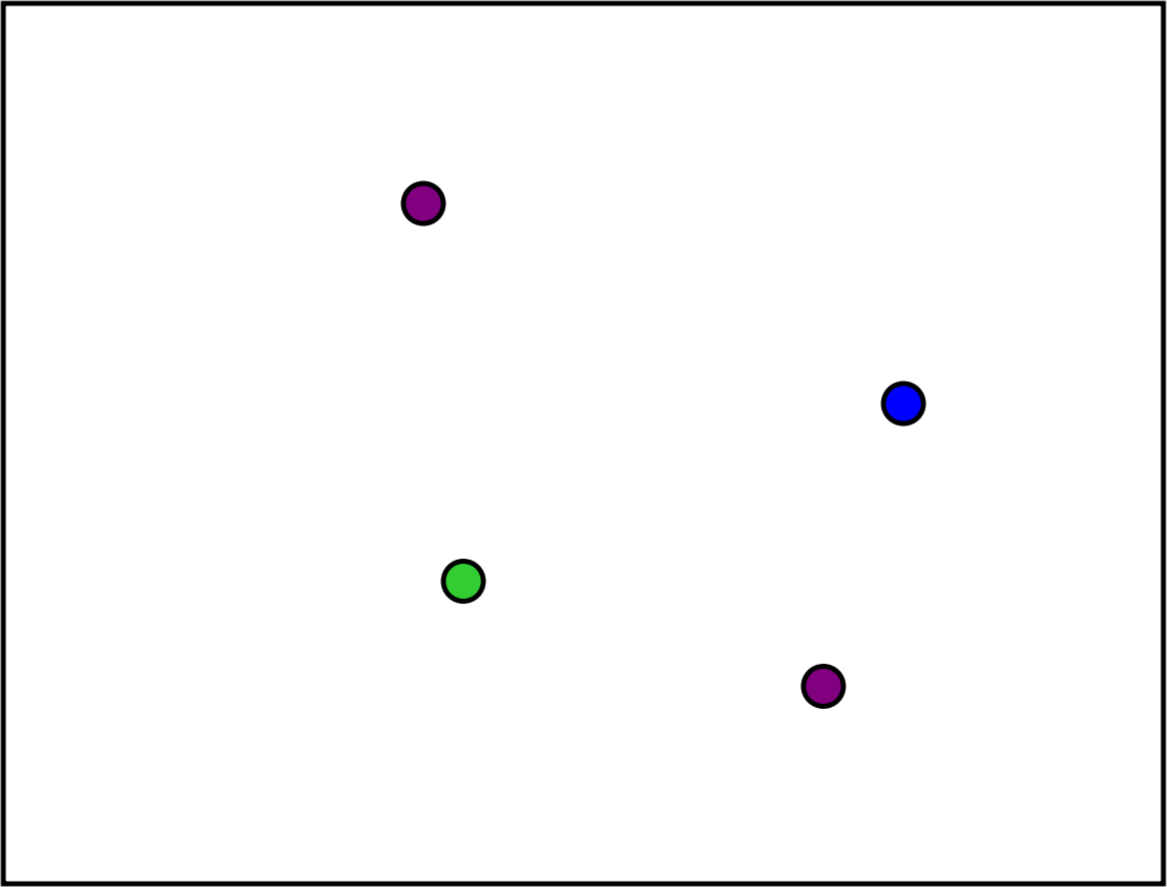
\includegraphics[width=5cm]{lucasKanade/retall2g.png}}\\


\caption{Optical flow example.}
\label{refArchiteOF}
\end{figure}

So, the question is: How do we estimate pixel motion from image $I(x,y,t)$ to image $I(x,y,t+1)$. We need to solve the pixel correspondence problem. Given a pixel in $I(x,y,t)$, look for nearby pixels of the same color in $I(x,y,t+1)$. Solving this problem is what is referred as the optical flow problem. By nearby pixels and same colour we have two assumptions:

\begin{itemize}

\item Colour constancy: a point in $I(x,y,t)$ looks the same in $I(x',y',t+1)$. For grayscale images, this is called \textit{Brightness constancy constraint}. Stated in mathematical formulation:

$$ I(x,y,t) = I(x+u,y+v,t+1) $$

$$ 0 = I(x+u,y+v,t+1)-I(x,y,t)  $$

\item Small motion: Subsequent points do not move very far, so we can estimate the motion by Taylor expansion: 

$$ I(x+u,y+v) 	\approx  I(x,y) + \dfrac{ \partial I}{\partial x}u +\dfrac{ \partial I}{\partial y}v + higher \hspace{0.1cm} order \hspace{0.1cm} terms $$


\end{itemize}
 
Then, combining these two equations, we get:

$$ 0 	\approx  I(x,y,t+1) + I_{x}u +I_{y}v - I(x,y,t) $$

where $I_{x} =  \dfrac{ \partial I}{\partial x}$, isolating the terms we obtain:

$$ 0 	\approx [I(x,y,t+1) - I(x,y,t)] + I_{x}u +I_{y}v $$

$$ 0 	\approx I_{t} + I_{x}u +I_{y}v $$

In the limit of $t$, $u$ and $v$ approaches zero ( assumption of small motion ), so it becomes, what it is called the the \textit{brightness constancy constraint equation}:
$$ 0 	= I_{t} + I_{x}u +I_{y}v $$

If we look closely, we realized that we have two unknowns $u,v$ and one equation. This is an underdetermined system. Intuitively, this means, that locally we can only determine the component of the flow in the gradient direction, the component of the flow parallel to an edge is unknown, this is the called the aperture problem. To recover the motion we need to add some extra constraints. There are several types of constraints to solve this problem:

\begin{itemize}

\item \textbf{Global constraint}, adding a smooth constraint to the brightness constraint, this new constraints penalizes for changes in $u$ and $v$ over the images, it assumes that the motion fields vary smoothly over the image. This approach was developed by Horn and Schunk \cite{horn}.

\item \textbf{Local constraint}, locally the motion field is almost the same, so we add the neighbours pixels to the equation. This approach was developed by Lucas and Kanade \cite{LucasKana}.
\end{itemize}



\textbf{Local constraint}

In this thesis we use the Local constraint to solve the optical flow problem. As we stated above, we add a local constraint to get more equations, this assumes that the motion field is the same in the locality. From the brightness constraint equation:

$$ 0 = I_{t}(p_{i}) + \nabla I(p_{i}) \hspace{0.1cm} [u \hspace{0.2cm} v]$$

Adding the neighborhood equations:

% 2

\[
\begin{bmatrix}
    I_{x}(p_{1}) & I_{y}(p_{1})  \\
    I_{x}(p_{2}) & I_{y}(p_{2})  \\
    \vdots & \vdots  \\
    I_{x}(p_{n}) & I_{y}(p_{n})
\end{bmatrix}
\begin{bmatrix}
    u \\
    v \\
\end{bmatrix}
=
\begin{bmatrix}
    -I_{t}(p_{1}) \\
    \vdots \\
    -I_{t}(p_{n}) \\
\end{bmatrix}
\]


Now, there are more equation than unknows, it is an overdetermined system, we have to solve it with the least squares technique. It is based on the optimization of the function:
%by using the pseudo inverse:
% 4
$$(A^{T}A) \hspace{0.1cm} d=A^{T} \hspace{0.1cm} b$$

Using the image notation:

% 5

\[
\begin{bmatrix}
    \sum I_{x}I_{x} & \sum I_{y}I_{x}  \\
    \sum I_{x}I_{y} & \sum I_{y}I_{y}   \\
\end{bmatrix}
\begin{bmatrix}
    u \\
    v \\
\end{bmatrix}
=
\begin{bmatrix}
    - \sum I_{x}I_{t} \\
    - \sum I_{y}I_{t} \\
\end{bmatrix}
\]



The system has a solution when $A^{t}A$ is invertible, it will be invertible when is well conditioned, this is when the ratio of the great and the small eigenvalues of the matrix is large but no too much. The matrix $A^{t}A$ in terms of image formulation is the second order matrix that we stated in the section \ref{feature} developing the \textit{cornerness}, then in order to be solvable it should have a strong gradient in both directions. After checking the invertability, we can solve the problem and extract the motion field:

% 6
$$ d = (A^{T}A)^{-1} \hspace{0.1cm}  A^{T}  \hspace{0.1cm} b  $$

Thus, using the image notation:

\[
\begin{bmatrix}
    u \\
    v \\
\end{bmatrix}
=
\begin{bmatrix}
    \sum I_{x}^{2} & \sum I_{y}I_{x}  \\
    \sum I_{x}I_{y} & \sum I_{y}^{2}   \\
\end{bmatrix}^{-1}
\begin{bmatrix}
    - \sum I_{x}I_{t} \\
    - \sum I_{y}I_{t} \\
\end{bmatrix}
\]



In practice motion is large, the assumption that it is small fails, consequently the approach using Taylor expansions. For two reasons, the linearity does not hold, in order to solve it, we apply an iterative refinement, which consists in compute the displacement, apply it to the pixels, and compute it again till it converges. The other one is there are local minimum and it will fail into it. To solve it, we need to utilize a coarse to fine approach, the idea is to use multiresolution to compute optical flow, the basic is that in a low resolution image the motion between pixels is very small and we can compute optical flow.

So, in order to do so, we use image pyramids, this consists in downsample these images to specific resolution, then in top level, we compute the motion field using the previous stated method, then 
we upsample the motion field and the images, We apply a transformation to one image according to the motion field computed in the previous level and then compute the optical flow between that 
transformed image and the other image, we apply this algorithm in all the resolutions

% image pyramids


\begin{figure}[H]
\centering         
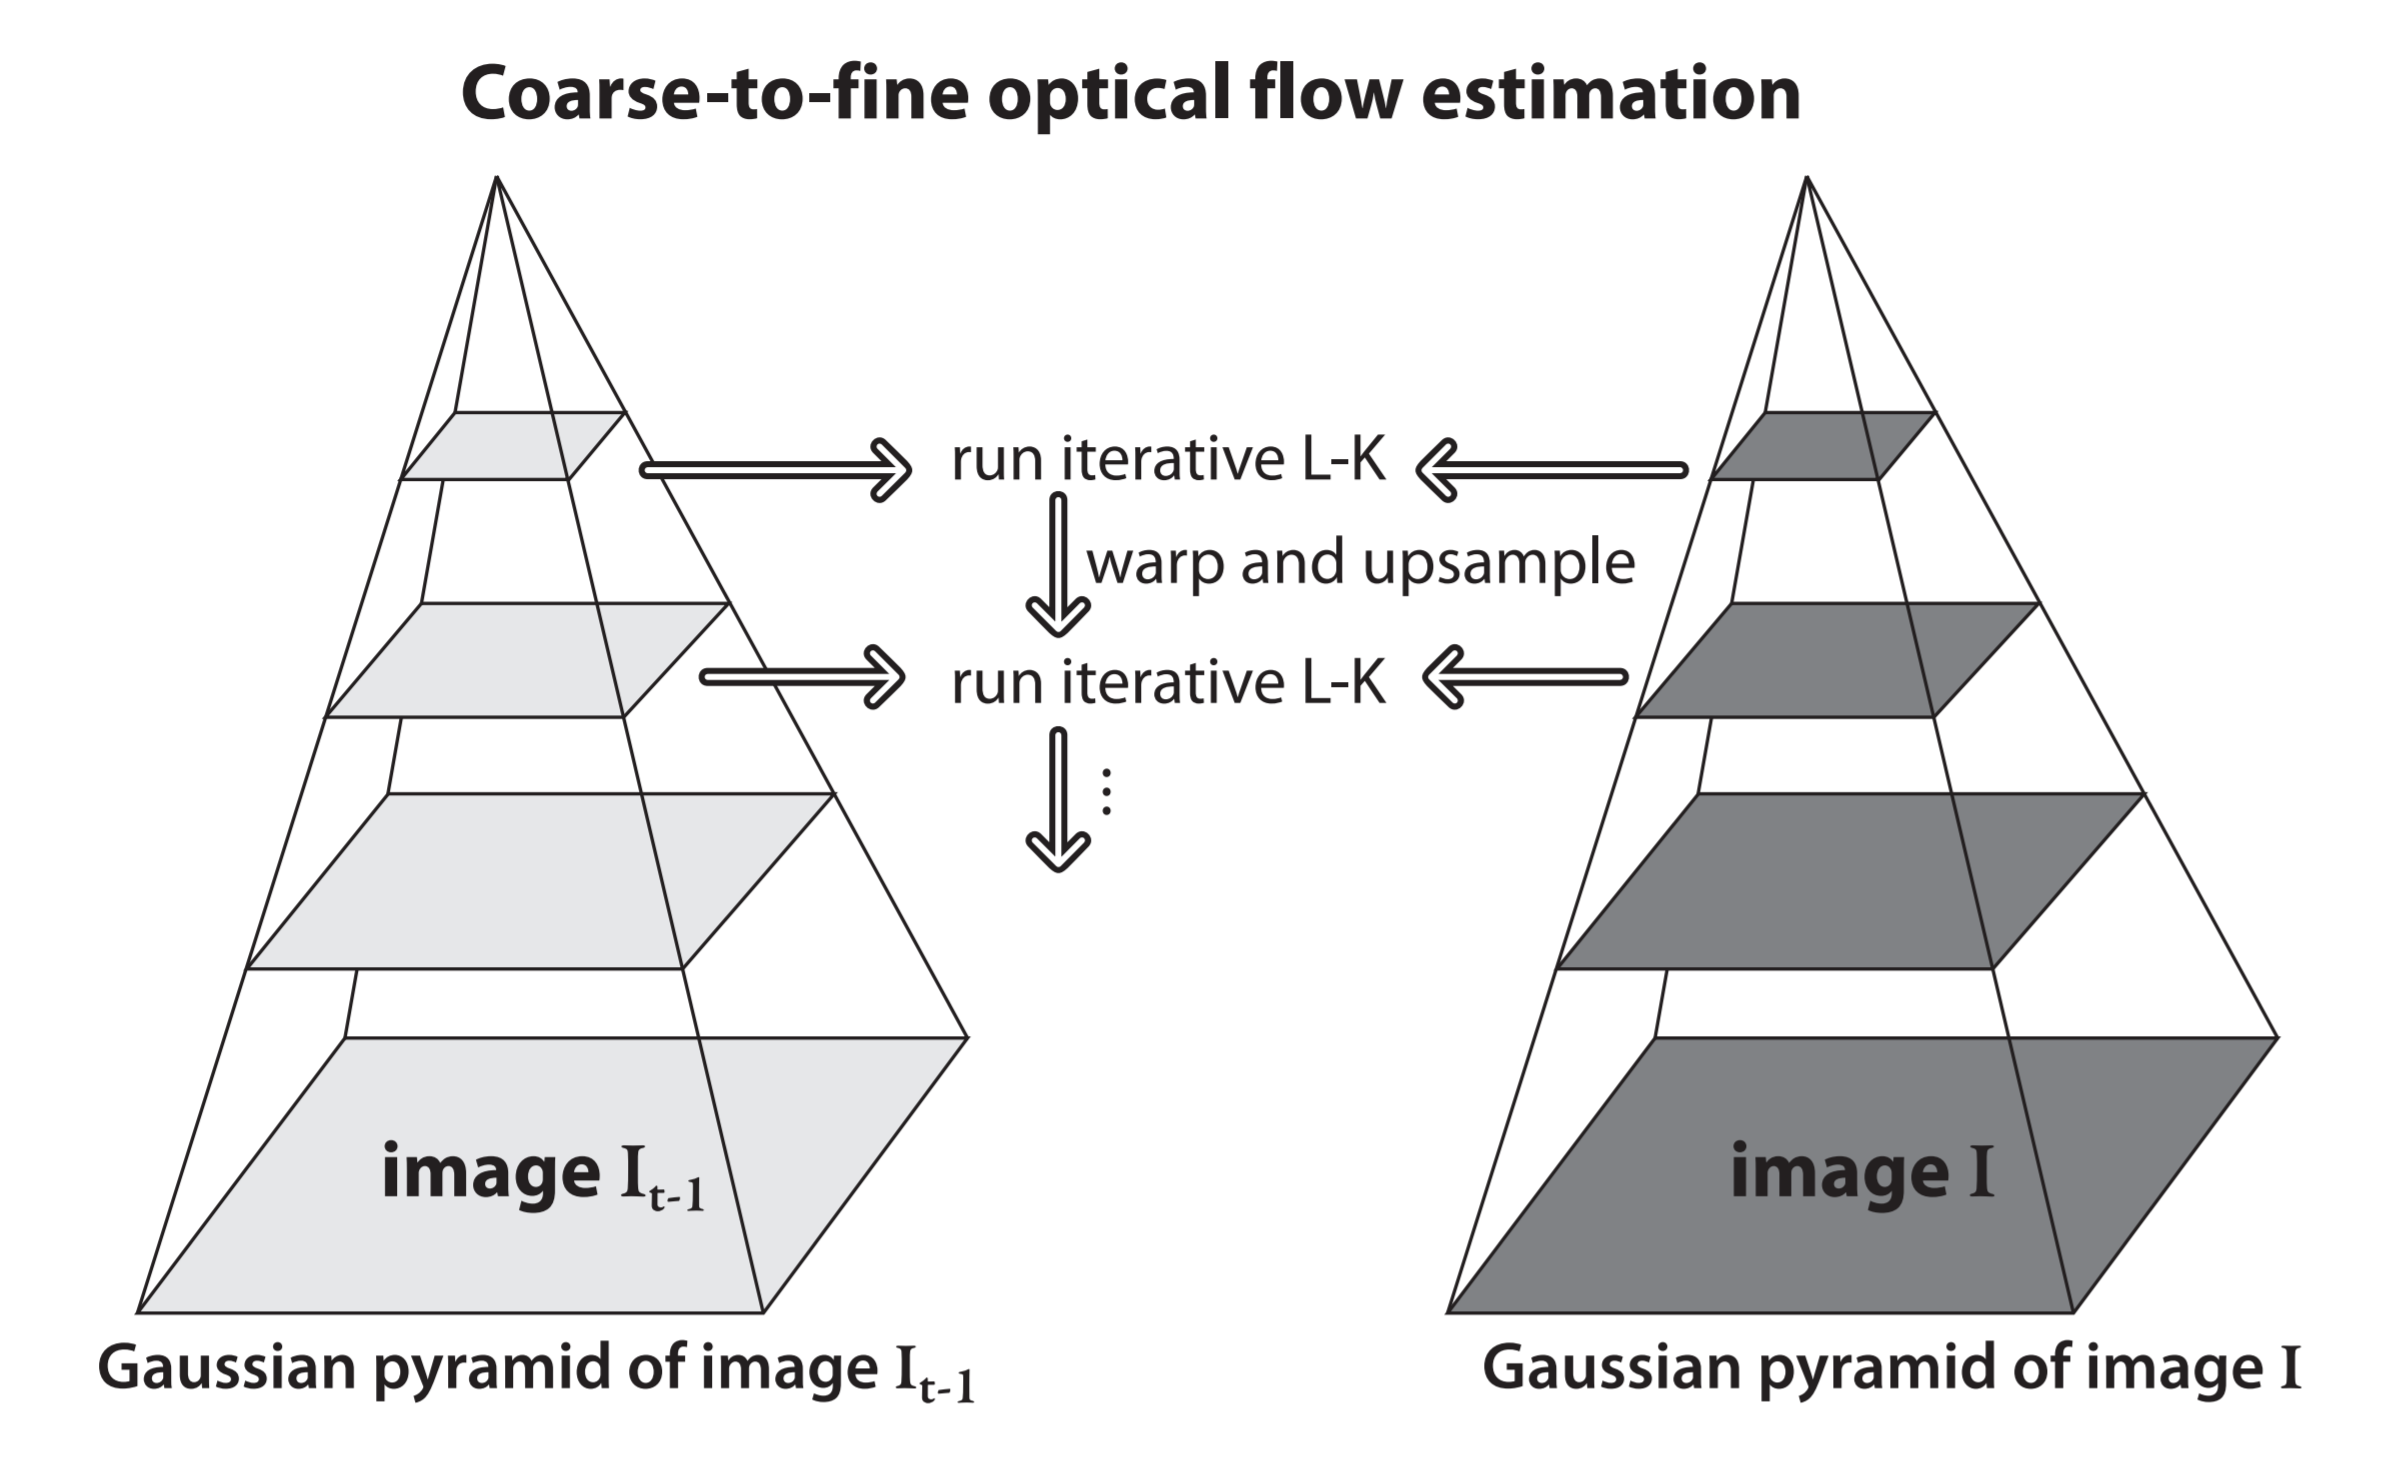
\includegraphics[width=0.6\linewidth]{lucasKanade/piram.png}
\caption{Optical flow with pyramids.} \label{corner}
\end{figure}





\section{Person re-Identification}\label{misMatch}


After running the tracking module we might lose some trackets and in the detection step we might recover them. We need a module to check whether these have the same identity. In order to do so, we studied the methods to recover the identity with deep learning techniques.

Person identification is thoroughly studied in the field of Biometrics, it consists of  knowing one biometric characteristic, and comparing with a claiming identity query. Specifically, the topic of pedestrian identification based on images has raised in the last years, this is due to the growth of surveillance applications. Also inside the topic of tracking there is a subfield called data association which studies this problem, it consists in matching trackets with further pedestrian detections.

Let's define mathematical the problem, consider $G$ is a gallery composed of $N$ images, denoted as $(g_{i})_{i=1}^{N}$. They belong to $N$ different identities $ 1,2,...,N $. Given a query image $q$, its identity is determined by:

%$$ i^{*} = argmax_{i \in 1,2,...,Ni \in 1,2,...,N} \hspace{0.5cm} sim(q,g_{i})$$

$$ i^{*} = \underset{i \in 1,2,...,N}{\arg\max} \hspace{0.5cm} sim(q,g_{i}) $$

where $i^{*}$ is the identity of probe $q$, and $sim( . , . )$ is some kind of similarity function. There are several categories of this similarity function \cite{pastPresent}:

\begin{itemize}
 
\item \textbf{Hand-crafted systems}. This involves two components, an image descriptor and a distance metric algorithm. The most common image descriptors are those used in computer vision too, like colour \cite{lbp}, texture \cite{pairwise}, SIFT \cite{sift}, bag of word \cite{bagword}. The general idea of distance metric learning is to keep all the vectors of the same class closer while pushing vectors of different classes further apart. The most commonly used formulation is based on the class of Mahalanobis distance function \cite{kiisme}, \cite{lnnn}. Other works focus on learning discriminative subspaces \cite{lda}.

\item \textbf{Deep learning techniques}. Two types of CNN models are commonly employed in the community, the first is the classification model as used in image classification, the output is an identity label, and the second one is the siamese model using image pairs as input. The major drawback of the classification models is that they need a great quantity of training data by category, and most of the identifications datasets only provide a few examples for identity. So currently methods focus on siamese models.

\end{itemize} 

The main differences between them, is that in hand-crafted methods, feature representation of the data and the metric are not learned jointly, instead, deep learning techniques jointly optimize the representation of the input data conditioned on the \textit{similarity} measure being used \cite{EC1}. 





\subsection{Siamese networks}



The first work with siamese architectures were developed by LeCun \cite{siamLecun}, \cite{siameLecun2} and they addressed the identification of signatures, besides the siamese networks are used in a variety of problems like: image recovery \cite{siameseQuer}, feature descriptor \cite{siameDescri}, comparing patches \cite{patch1}, one shot learning \cite{siameseOne}, and learning visual similarity \cite{siamesSImi}. 

Siamese CNN topologies can be grouped under three main categories, depending on the point where the information from each input is combined:

\begin{itemize}

\item \textbf{Cost function}. Input patches are processed by two parallel branches featuring the same network structure and weights. Finally, the top layers of each branch are fed to a cost function.

\item \textbf{In-network}. The top layers of the parallel branches processing the two different inputs are concatenated and some more layers added on top of that.

\item \textbf{Joint data input}. The two input patches are stacked together forming a unified input to the CNN.

\end{itemize}

Graphical we can observe those differences in \ref{siamese2Data1}.
\begin{figure}[H]
		
\centering

\subfigure[Cost function.]{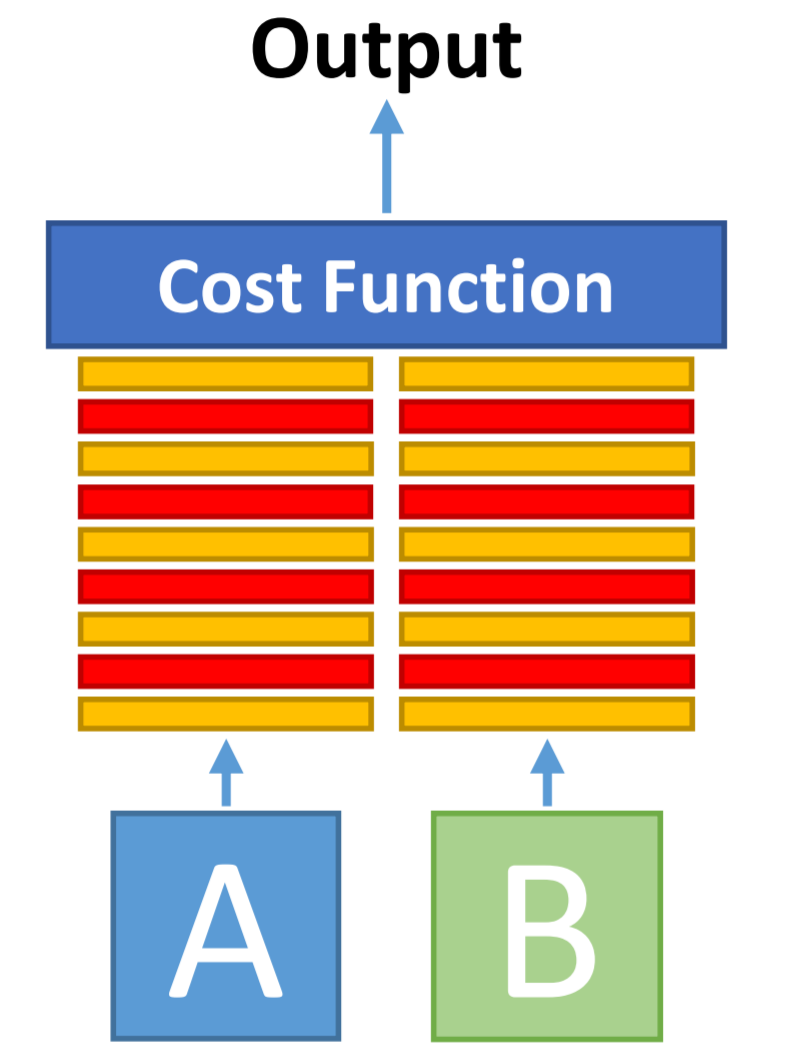
\includegraphics[width=2.7cm]{siamese/retall1.png}}
\subfigure[In-network.]{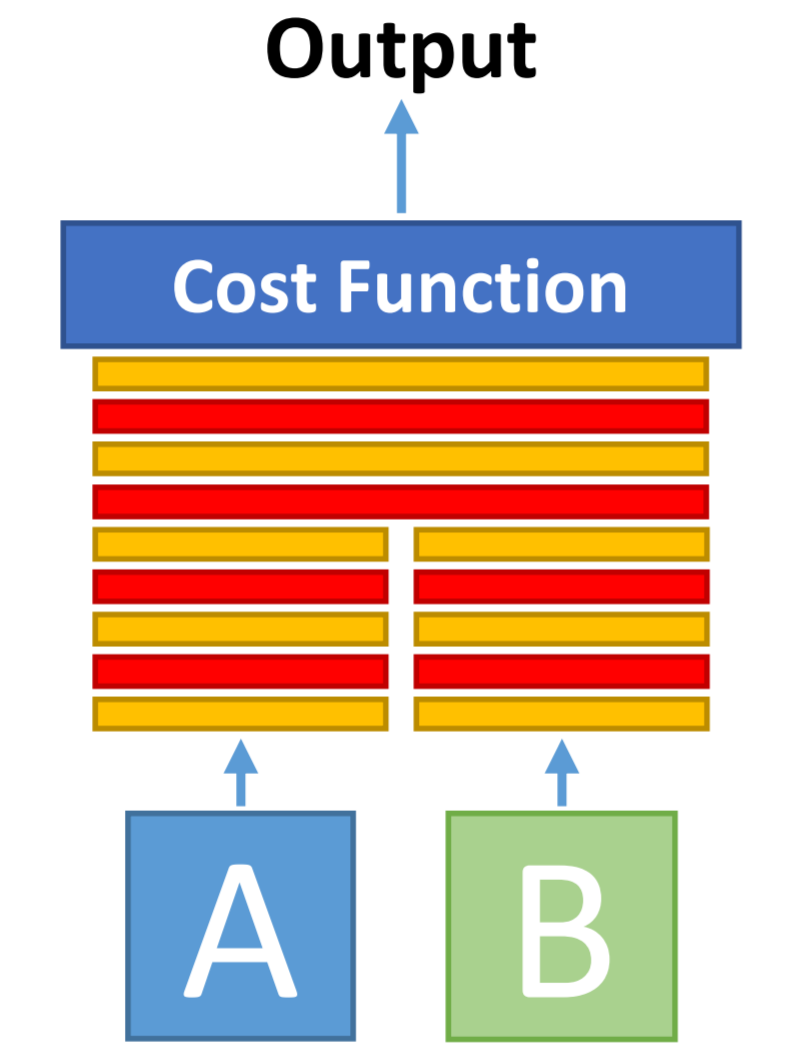
\includegraphics[width=2.7cm]{siamese/retall2.png}}
\subfigure[Joint data input.]{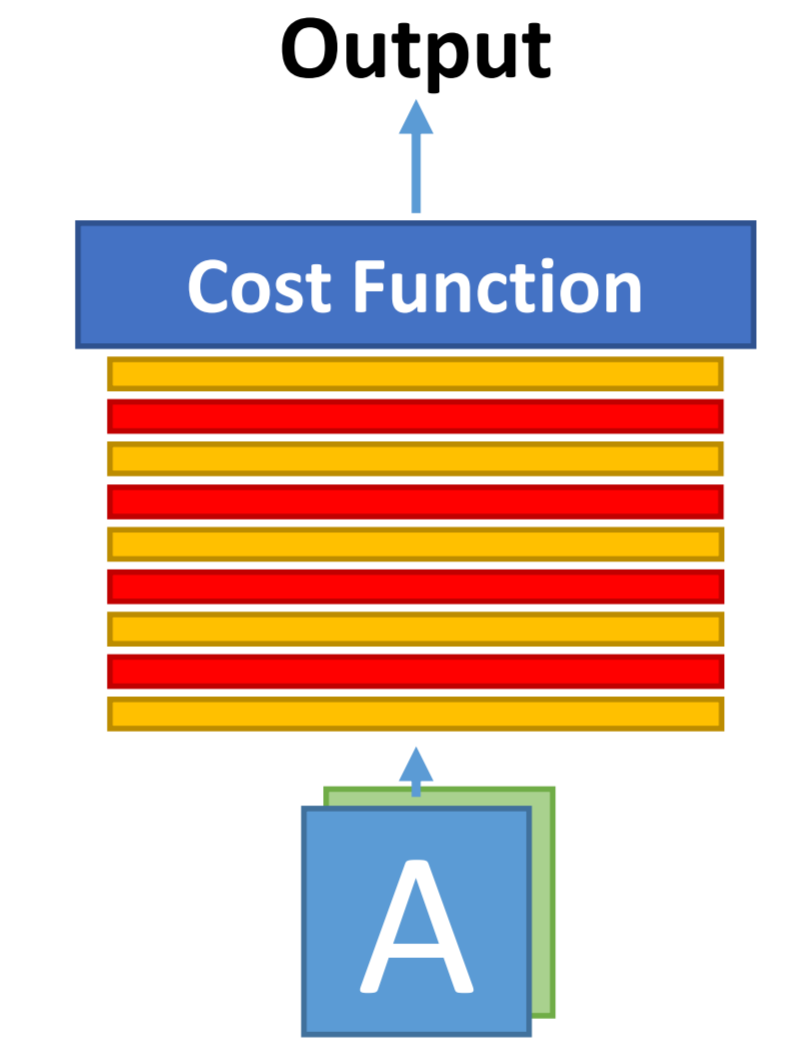
\includegraphics[width=2.7cm]{siamese/retall3.png}}

\caption{Siamese CNN topologies.}
\label{siamese2Data1}
\end{figure}


While the two first approaches have yield good results and historically were dominant, the best performance is obtained with the joint data input strategy. As pointed out by  \cite{patch1} and further corroborated by \cite{patch2}, and \cite{patch3}, jointly using information form both images from the first layer tends to deliver a better performance. 


In the field of person re-identification, the community has used these architectures, and they also, have developed their own loss function, what is called \textit{contrastive loss}, this loss is an extension of the Hinge loss of the SVM. This loss longs for getting close similar pairs and moving away according to one defined margin, dissimilar pairs. Although, the binary cross entropy is used by the community. Also, the community has focused in the developing of the datasets, increase the size and quality but there are not any landmark dataset.


There are several papers in the literature, one of the most famous is developed by Ahmed \cite{ahmed}, they used In-network architecture although in order to join to the convolutional layers, they used \textit{cross-input neighborhood differences} layer, this layer tried to increase the differences between the features of the inputs and obtain richer representation to the classification layer.

Another paper was published by Leal-Taixé \cite{lealTaixe}, they are also the authors of the MOT challenge, their network used a cost function architecture besides they used as inputs the two images and their optical flow. They used the network as part of a data association algorithm.


